\documentclass[table]{hfstyle/hf}

% Basic packages
\usepackage[utf8]{inputenc}
\usepackage[T1]{fontenc}
\usepackage{graphicx}
\usepackage{booktabs}
\usepackage{url}
\usepackage{lineno}
\usepackage{enumitem}
\usepackage{listings}

% Math and symbols
\usepackage{amsmath}
\usepackage{amsfonts}
\usepackage{amssymb}
\usepackage{nicefrac}
\usepackage{siunitx}

% Tables and figures
\usepackage{multirow}
\usepackage{bigdelim}
\usepackage{longtable}
\usepackage{tabularray}
\usepackage{wrapfig}
\usepackage{caption}
% \usepackage{subcaption}  % Commented out - add back when using subfigures
\usepackage{makecell}
\usepackage{adjustbox}

% Color and boxes
\usepackage[most]{tcolorbox}
\usepackage{xcolor}

% Text and formatting
\usepackage{xspace}
\usepackage{soul}
\usepackage{csquotes}
\usepackage{arydshln}

% Bibliography and references
\usepackage{natbib}

% Special packages
\usepackage{todonotes}
\usepackage[absolute]{textpos}
\usepackage{pifont}
\usepackage{bold-extra}
\usepackage{pgf-pie}
\usepackage{epigraph}

% Algorithms
\usepackage{algorithm}
\usepackage{algpseudocode}

% Hyperref (load last)
\usepackage{hyperref}
\definecolor{linkcolor}{RGB}{0, 0, 128}
\hypersetup{
     colorlinks   = true,
     citecolor    = linkcolor,
     linkcolor    = linkcolor,
     urlcolor     = linkcolor,
}

% Custom commands
\newcommand{\cmark}{\ding{51}}%
\newcommand{\xmark}{\ding{55}}%

\setlist[itemize]{leftmargin=*,itemsep=0em,parsep=0.3em,topsep=0.3em}

\DeclareUnicodeCharacter{2212}{\ensuremath{-}}

\addtolength{\extrarowheight}{\belowrulesep}
\aboverulesep=0pt
\belowrulesep=0pt

\definecolor{maroon}{HTML}{F26035}
\definecolor{yellow}{HTML}{FDBC42}
\definecolor{lavender}{HTML}{734f96}
\definecolor{darkergrey}{HTML}{444444}
\definecolor{midgrey}{HTML}{e6eded}

\definecolor{neutralEight}{HTML}{343434}
\definecolor{neutralFive}{HTML}{838383}
\definecolor{neutralThree}{HTML}{bebebe}
\definecolor{neutralOne}{HTML}{dedede}
\definecolor{lightgrey}{HTML}{fafcfc}

\usepackage{tikz}
\newcommand{\cblock}[3]{
  \hspace{-1.5mm}
  \begin{tikzpicture}
    [
    node/.style={square, minimum size=10mm, thick, line width=0pt},
    ]
    \node[fill={rgb,255:red,#1;green,#2;blue,#3}] () [] {};
  \end{tikzpicture}%
}

\newcommand{\norm}[1]{\left\lVert#1\right\rVert}

\definecolor{maroon}{HTML}{F26035}
\definecolor{yellow}{HTML}{FDBC42}
\definecolor{darkred}{RGB}{156, 39, 33}
\definecolor{darkblue}{RGB}{31, 90, 153}
\definecolor{forestgreen}{rgb}{0.13, 0.55, 0.13}
\definecolor{olmoDarkBlue}{HTML}{012e59}
\definecolor{olmoBlue}{HTML}{265ed4}
\definecolor{olmoLightBlue}{HTML}{012e59}
\definecolor{olmoTeal}{HTML}{00d5ff}
\definecolor{olmoYellow}{HTML}{ffbb00}
\definecolor{olmoOrange}{HTML}{ff9100}


\newcommand{\nol}[1]{{\color{purple} [nol]: #1}}


\usepackage{setspace}

\usepackage{nicematrix}
\newcolumntype{L}[1]{>{\raggedright\let\newline\\\arraybackslash\hspace{0pt}}m{#1}}
\newcolumntype{C}[1]{>{\centering\let\newline\\\arraybackslash\hspace{0pt}}m{#1}}
\newcolumntype{R}[1]{>{\raggedleft\let\newline\\\arraybackslash\hspace{0pt}}m{#1}}
\newcolumntype{P}[1]{>{\centering\let\newline\\\arraybackslash\columncolor{ai2lightpink}}m{#1}}
\addtolength{\extrarowheight}{\belowrulesep}
\aboverulesep=0pt
\belowrulesep=0pt

\newcommand{\orr}[1]{\textcolor{red}{[OZ:#1]}}


\definecolor{lightyellow}{rgb}{1, 0.95, 0.85}
\definecolor{graphicbackground}{rgb}{0.9765,0.9451,0.9059}
\definecolor{codebackground}{rgb}{0.8314,0.949,0.9882}

\newcommand{\finding}[2]{%
  \begin{tcolorbox}[colback=lightyellow, colframe=black, arc=4pt, boxsep=1pt]
    \paragraph{\textbf{\textit{Finding} #1.}} #2
  \end{tcolorbox}%
}

% Tables - packages already loaded in main.tex
% \usepackage{booktabs}
% \usepackage{graphicx}
% \usepackage{subfig}
% \usepackage{subcaption}
% \usepackage{multirow}

\newcommand{\tablestyle}[2]{\setlength{\tabcolsep}{#1}\renewcommand{\arraystretch}{#2}\centering\footnotesize}
\newlength\savewidth\newcommand\shline{\noalign{\global\savewidth\arrayrulewidth
  \global\arrayrulewidth 1pt}\hline\noalign{\global\arrayrulewidth\savewidth}}

\newlength\thinwidth\newcommand\thinline{\noalign{\global\savewidth\arrayrulewidth
  \global\arrayrulewidth 0.5pt}\hline\noalign{\global\arrayrulewidth\savewidth}}

\definecolor{Gray}{gray}{0.92}
\definecolor{DarkGray}{gray}{0.5}

% colors
\definecolor{LightCyan}{rgb}{0.88,1,1}
\definecolor{altRowColor}{gray}{0.92}
\definecolor{highlightRowColor}{rgb}{0.9, 0.9, 1}
\newcommand{\colorrow}{\rowcolor{highlightRowColor}}
\newcommand{\grayrow}{\rowcolor{Gray}}
\newcommand{\highlightcell}{\cellcolor{highlightRowColor}}
\newcommand{\colorcell}{\cellcolor{Gray}}


\newcommand{\cpar}{\par\noindent\textbf}

\newcommand{\graytext}{\textcolor{gray}}


\newcommand{\Mus}[1]{{\color{red}\textbf{Mus:#1}}}
\newcommand{\Dan}[1]{{\color{blue}\textbf{Dana:#1}}}


\newcommand{\ours}{{SmolVLA}\xspace}
\newcommand*\diff{\mathrm{d}}
\newcommand*\Image{\mathrm{Im}}
\newcommand*\NN{\smash{\hat{\mathcal{F}}_{\scriptsize\textrm{NN}}}}

\newcommand*\X{\mathcal{X}}
\newcommand*\Z{\mathcal{Z}}
\newcommand*\G{\mathcal{G}}
\newcommand*\D{\mathcal{D}}
\newcommand*\F{\mathcal{F}}
\newcommand*\R{\mathcal{R}}
\newcommand*\TR{\hat{R}}
\newcommand*\Deltab{\bar{\Delta}}
\newcommand*\h{h}
\newcommand*\biasb{\mathrm{bias}}
\newcommand*\varb{\mathrm{var}}
\newcommand*\covb{\mathrm{cov}}
\newcommand*\M{\mathcal{M}}
\newcommand*\B{\mathcal{B}}
\newcommand*\W{\mathcal{W}}
\newcommand*\Loss{\mathcal{L}}
\newcommand*{\Ftr}{\smash{\mathcal{F}_{\scriptsize\textrm{tr}}}}
\newcommand*{\Fts}{\smash{\mathcal{F}_{\scriptsize\textrm{ad}}}}
\newcommand*{\Dtr}{\smash{\mathcal{D}_{\scriptsize\textrm{tr}}}}
\newcommand*{\Dts}{\smash{\mathcal{D}_{\scriptsize\textrm{ad}}}}
\newcommand*{\Etr}{\smash{\mathcal{E}_{\scriptsize\textrm{tr}}}}
\newcommand*{\Ead}{\smash{\mathcal{E}_{\scriptsize\textrm{ad}}}}

\newcommand*{\eg}{e.g.,\@\xspace}
\newcommand*{\versus}{vs.\@\xspace}
\newcommand*{\sut}{s.t.\@\xspace}
\newcommand*{\ie}{i.e.,\@\xspace}
\newcommand*{\iid}{ID\@\xspace}
\newcommand*{\sota}{SoTA\@\xspace}
\newcommand*{\ood}{OOD\@\xspace}
\newcommand*{\metric}{metric}
\newcommand*{\wrt}{w.r.t.\@\xspace}
\newcommand*{\iif}{i.i.f.\@\xspace}
\newcommand*{\aka}{a.k.a.\@\xspace}
\newcommand*{\rhs}{r.h.s.\@\xspace}
\newcommand*{\etc}{etc.\@\xspace}
\newcommand*{\cf}{cf.\@\xspace}
\newcommand*{\resp}{resp.\@\xspace}

\newcommand*\er{\mathrm{er}}
\newcommand*\ess{\operatorname{ess}}

\let\originalleft\left
\let\originalright\right
\renewcommand{\left}{\mathopen{}\mathclose\bgroup\originalleft}
\renewcommand{\right}{\aftergroup\egroup\originalright}

\let\up\textsuperscript
\let\vec\boldsymbol


\newcommand{\defeq}{\mathrel{:\mkern-0.25mu=}}
\newcommand{\eqdef}{\mathrel{=\mkern-0.25mu:}}

\newcommand{\figleft}{{\em (Left)}}
\newcommand{\figcenter}{{\em (Center)}}
\newcommand{\figright}{{\em (Right)}}
\newcommand{\figtop}{{\em (Top)}}
\newcommand{\figbottom}{{\em (Bottom)}}
\newcommand{\captiona}{{\em (a)}}
\newcommand{\captionb}{{\em (b)}}
\newcommand{\captionc}{{\em (c)}}
\newcommand{\captiond}{{\em (d)}}

\newcommand{\newterm}[1]{{\bf #1}}
\def\figref#1{figure~\ref{#1}}
\def\Figref#1{Figure~\ref{#1}}
\def\twofigref#1#2{figures \ref{#1} and \ref{#2}}
\def\trifigref#1#2#3#4{figures \ref{#1}, \ref{#2}, and \ref{#3}}
\def\quadfigref#1#2#3#4{figures \ref{#1}, \ref{#2}, \ref{#3} and \ref{#4}}
\def\secref#1{section~\ref{#1}}
\def\Secref#1{Section~\ref{#1}}
\def\Termref#1{Term~\ref{#1}}
\def\twosecref#1#2{sections \ref{#1} and \ref{#2}}
\def\trisecref#1#2#3{sections \ref{#1}, \ref{#2} and \ref{#3}}
\def\appref#1{appendix~\ref{#1}}
\def\Appref#1{Appendix~\ref{#1}}
\def\suppref#1{supp.~\ref{#1}}
\def\Suppref#1{Supp.~\ref{#1}}
\def\eqref#1{eq.~\ref{#1}}
\def\Eqref#1{Eq.~\ref{#1}}
\def\plaineqref#1{\ref{#1}}
\def\chapref#1{chapter~\ref{#1}}
\def\Chapref#1{Chapter~\ref{#1}}
\def\rangechapref#1#2{chapters\ref{#1}--\ref{#2}}
\def\algref#1{algorithm~\ref{#1}}
\def\Algref#1{Algorithm~\ref{#1}}
\def\twoalgref#1#2{algorithms \ref{#1} and \ref{#2}}
\def\Twoalgref#1#2{Algorithms \ref{#1} and \ref{#2}}
\def\partref#1{part~\ref{#1}}
\def\Partref#1{Part~\ref{#1}}
\def\twopartref#1#2{parts \ref{#1} and \ref{#2}}

\def\Tabref#1{Table~\ref{#1}}
\def\tabref#1{table~\ref{#1}}
\def\twotabref#1#2{tables \ref{#1} and \ref{#2}}

\def\ceil#1{\lceil #1 \rceil}
\def\floor#1{\lfloor #1 \rfloor}

\newcommand{\Lp}{\mathcal{L}^\text{prior}}
\newcommand{\Ll}{\mathcal{L}^\text{likeli}}
\newcommand{\Lal}{\Ls^{\text{l}\widehat{\text{ikel}}\text{i}}}

\def\eps{{\varepsilon}}


\def\xopt{{x^{*}}}
\def\Gopt{{G^{*}}}

\def\p{{\textnormal{p}}}
\def\P{{\textnormal{p}}}
\def\Q{{\textnormal{q}}}
\def\q{{\textnormal{q}}}

\def\gTh{{\hat \gT}}
\def\gDh{{\hat \gD}}
\def\gPh{{\hat \gP}}
\newcommand{\tin}[1]{\mbox{\tiny $#1$}}


\def\reta{{\textnormal{$\eta$}}}
\def\ra{{\textnormal{a}}}
\def\rb{{\textnormal{b}}}
\def\rc{{\textnormal{c}}}
\def\rd{{\textnormal{d}}}
\def\re{{\textnormal{e}}}
\def\rf{{\textnormal{f}}}
\def\rg{{\textnormal{g}}}
\def\rh{{\textnormal{h}}}
\def\ri{{\textnormal{i}}}
\def\rj{{\textnormal{j}}}
\def\rk{{\textnormal{k}}}
\def\rl{{\textnormal{l}}}
\def\rn{{\textnormal{n}}}
\def\ro{{\textnormal{o}}}
\def\rp{{\textnormal{p}}}
\def\rq{{\textnormal{q}}}
\def\rr{{\textnormal{r}}}
\def\rs{{\textnormal{s}}}
\def\rt{{\textnormal{t}}}
\def\ru{{\textnormal{u}}}
\def\rv{{\textnormal{v}}}
\def\rw{{\textnormal{w}}}
\def\reps{{\mathcal{E}}}
\def\rtheta{{\Theta}}
\def\rx{{X}}
\def\ry{{Y}}
\def\rz{{Z}}


\def\S{\mathcal{S}}
\def\T{\mathcal{T}}
\def\X{\mathcal{X}}
\def\Y{\mathcal{Y}}
\def\U{\mathcal{U}}

\def\rvepsilon{{\mathbf{\epsilon}}}
\def\rva{{\mathbf{a}}}
\def\rvb{{\mathbf{b}}}
\def\rvc{{\mathbf{c}}}
\def\rvd{{\mathbf{d}}}
\def\rve{{\mathbf{e}}}
\def\rvf{{\mathbf{f}}}
\def\rvg{{\mathbf{g}}}
\def\rvh{{\mathbf{h}}}
\def\rvu{{\mathbf{i}}}
\def\rvj{{\mathbf{j}}}
\def\rvk{{\mathbf{k}}}
\def\rvl{{\mathbf{l}}}
\def\rvm{{\mathbf{m}}}
\def\rvn{{\mathbf{n}}}
\def\rvo{{\mathbf{o}}}
\def\rvp{{\mathbf{p}}}
\def\rvq{{\mathbf{q}}}
\def\rvr{{\mathbf{r}}}
\def\rvs{{\mathbf{s}}}
\def\rvt{{\mathbf{t}}}
\def\rvu{{\mathbf{u}}}
\def\rvv{{\mathbf{v}}}
\def\rvw{{\mathbf{w}}}
\def\rvx{{\mathbf{x}}}
\def\rvy{{\mathbf{y}}}
\def\rvz{{\mathbf{z}}}
\def\rvtheta{{\bm{\theta}}}

\def\erva{{\textnormal{a}}}
\def\ervb{{\textnormal{b}}}
\def\ervc{{\textnormal{c}}}
\def\ervd{{\textnormal{d}}}
\def\erve{{\textnormal{e}}}
\def\ervf{{\textnormal{f}}}
\def\ervg{{\textnormal{g}}}
\def\ervh{{\textnormal{h}}}
\def\ervi{{\textnormal{i}}}
\def\ervj{{\textnormal{j}}}
\def\ervk{{\textnormal{k}}}
\def\ervl{{\textnormal{l}}}
\def\ervm{{\textnormal{m}}}
\def\ervn{{\textnormal{n}}}
\def\ervo{{\textnormal{o}}}
\def\ervp{{\textnormal{p}}}
\def\ervq{{\textnormal{q}}}
\def\ervr{{\textnormal{r}}}
\def\ervs{{\textnormal{s}}}
\def\ervt{{\textnormal{t}}}
\def\ervu{{\textnormal{u}}}
\def\ervv{{\textnormal{v}}}
\def\ervw{{\textnormal{w}}}
\def\ervx{{\textnormal{x}}}
\def\ervy{{\textnormal{y}}}
\def\ervz{{\textnormal{z}}}

\def\rmA{{\mathbf{A}}}
\def\rmB{{\mathbf{B}}}
\def\rmC{{\mathbf{C}}}
\def\rmD{{\mathbf{D}}}
\def\rmE{{\mathbf{E}}}
\def\rmF{{\mathbf{F}}}
\def\rmG{{\mathbf{G}}}
\def\rmH{{\mathbf{H}}}
\def\rmI{{\mathbf{I}}}
\def\rmJ{{\mathbf{J}}}
\def\rmK{{\mathbf{K}}}
\def\rmL{{\mathbf{L}}}
\def\rmM{{\mathbf{M}}}
\def\rmN{{\mathbf{N}}}
\def\rmO{{\mathbf{O}}}
\def\rmP{{\mathbf{P}}}
\def\rmQ{{\mathbf{Q}}}
\def\rmR{{\mathbf{R}}}
\def\rmS{{\mathbf{S}}}
\def\rmT{{\mathbf{T}}}
\def\rmU{{\mathbf{U}}}
\def\rmV{{\mathbf{V}}}
\def\rmW{{\mathbf{W}}}
\def\rmx{{\mathbf{x}}}
\def\rmy{{\mathbf{y}}}
\def\rmz{{\mathbf{Z}}}

\def\ermA{{\textnormal{A}}}
\def\ermB{{\textnormal{B}}}
\def\ermC{{\textnormal{C}}}
\def\ermD{{\textnormal{D}}}
\def\ermE{{\textnormal{E}}}
\def\ermF{{\textnormal{F}}}
\def\ermG{{\textnormal{G}}}
\def\ermH{{\textnormal{H}}}
\def\ermI{{\textnormal{I}}}
\def\ermJ{{\textnormal{J}}}
\def\ermK{{\textnormal{K}}}
\def\ermL{{\textnormal{L}}}
\def\ermM{{\textnormal{M}}}
\def\ermN{{\textnormal{N}}}
\def\ermO{{\textnormal{O}}}
\def\ermP{{\textnormal{P}}}
\def\ermQ{{\textnormal{Q}}}
\def\ermR{{\textnormal{R}}}
\def\ermS{{\textnormal{S}}}
\def\ermT{{\textnormal{T}}}
\def\ermU{{\textnormal{U}}}
\def\ermV{{\textnormal{V}}}
\def\ermW{{\textnormal{W}}}
\def\ermX{{\textnormal{X}}}
\def\ermY{{\textnormal{Y}}}
\def\ermZ{{\textnormal{Z}}}

\def\vzero{{\bm{0}}}
\def\vone{{\bm{1}}}
\def\va{{\bm{a}}}
\def\vb{{\bm{b}}}
\def\vc{{\bm{c}}}
\def\vd{{\bm{d}}}
\def\ve{{\bm{e}}}
\def\vf{{\bm{f}}}
\def\vg{{\bm{g}}}
\def\vh{{\bm{h}}}
\def\vi{{\bm{i}}}
\def\vj{{\bm{j}}}
\def\vk{{\bm{k}}}
\def\vl{{\bm{l}}}
\def\vm{{\bm{m}}}
\def\vn{{\bm{n}}}
\def\vo{{\bm{o}}}
\def\vp{{\bm{p}}}
\def\vq{{\bm{q}}}
\def\vr{{\bm{r}}}
\def\vs{{\bm{s}}}
\def\vt{{\bm{t}}}
\def\vu{{\bm{u}}}
\def\vv{{\bm{v}}}
\def\vw{{\bm{w}}}
\def\vx{{\bm{x}}}
\def\vy{{\bm{y}}}
\def\vz{{\bm{z}}}
\def\valpha{{\bm{\alpha}}}
\def\vtheta{{\bm{\theta}}}
\def\vdelta{{\bm{\delta}}}
\def\vDelta{{\bm{\Delta}}}
\def\vmu{{\bm{\mu}}}
\def\vphi{{\bm{\phi}}}
\def\vSigma{{\bm{\Sigma}}}
\def\evalpha{{\alpha}}
\def\evbeta{{\beta}}
\def\evepsilon{{\epsilon}}
\def\evlambda{{\lambda}}
\def\evomega{{\omega}}
\def\evmu{{\mu}}
\def\evpsi{{\psi}}
\def\evsigma{{\sigma}}
\def\evtheta{{\theta}}
\def\eva{{a}}
\def\evb{{b}}
\def\evc{{c}}
\def\evd{{d}}
\def\eve{{e}}
\def\evf{{f}}
\def\evg{{g}}
\def\evh{{h}}
\def\evi{{i}}
\def\evj{{j}}
\def\evk{{k}}
\def\evl{{l}}
\def\evm{{m}}
\def\evn{{n}}
\def\evo{{o}}
\def\evp{{p}}
\def\evq{{q}}
\def\evr{{r}}
\def\evs{{s}}
\def\evt{{t}}
\def\evu{{u}}
\def\evv{{v}}
\def\evw{{w}}
\def\evx{{x}}
\def\evy{{y}}
\def\evz{{z}}

\def\mA{{\bm{A}}}
\def\mB{{\bm{B}}}
\def\mC{{\bm{C}}}
\def\mD{{\bm{D}}}
\def\mE{{\bm{E}}}
\def\mF{{\bm{F}}}
\def\mG{{\bm{G}}}
\def\mH{{\bm{H}}}
\def\mI{{\bm{I}}}
\def\mJ{{\bm{J}}}
\def\mK{{\bm{K}}}
\def\mL{{\bm{L}}}
\def\mM{{\bm{M}}}
\def\mN{{\bm{N}}}
\def\mO{{\bm{O}}}
\def\mP{{\bm{P}}}
\def\mQ{{\bm{Q}}}
\def\mR{{\bm{R}}}
\def\mS{{\bm{S}}}
\def\mT{{\bm{T}}}
\def\mU{{\bm{U}}}
\def\mV{{\bm{V}}}
\def\mW{{\bm{W}}}
\def\mX{{\bm{X}}}
\def\mY{{\bm{Y}}}
\def\mZ{{\bm{Z}}}
\def\E{{\mathcal{E}}}
\def\mBeta{{\bm{\beta}}}
\def\mTheta{{\bm{\theta}}}
\def\mPhi{{\bm{\Phi}}}
\def\mLambda{{\bm{\Lambda}}}
\def\mSigma{{\bm{\Sigma}}}

\DeclareMathAlphabet{\mathsfit}{\encodingdefault}{\sfdefault}{m}{sl}
\SetMathAlphabet{\mathsfit}{bold}{\encodingdefault}{\sfdefault}{bx}{n}
\newcommand{\tens}[1]{\bm{\mathsfit{#1}}}
\def\tA{{\tens{A}}}
\def\tB{{\tens{B}}}
\def\tC{{\tens{C}}}
\def\tD{{\tens{D}}}
\def\tE{{\tens{E}}}
\def\tF{{\tens{F}}}
\def\tG{{\tens{G}}}
\def\tH{{\tens{H}}}
\def\tI{{\tens{I}}}
\def\tJ{{\tens{J}}}
\def\tK{{\tens{K}}}
\def\tL{{\tens{L}}}
\def\tM{{\tens{M}}}
\def\tN{{\tens{N}}}
\def\tO{{\tens{O}}}
\def\tP{{\tens{P}}}
\def\tQ{{\tens{Q}}}
\def\tR{{\tens{R}}}
\def\tS{{\tens{S}}}
\def\tT{{\tens{T}}}
\def\tU{{\tens{U}}}
\def\tV{{\tens{V}}}
\def\tW{{\tens{W}}}
\def\tX{{\tens{X}}}
\def\tY{{\tens{Y}}}
\def\tZ{{\tens{Z}}}

\def\tx{{\tens{x}}}


\def\gA{{\mathcal{A}}}
\def\gB{{\mathcal{B}}}
\def\gC{{\mathcal{C}}}
\def\gD{{\mathcal{D}}}
\def\gE{{\mathcal{E}}}
\def\gF{{\mathcal{F}}}
\def\gG{{\mathcal{G}}}
\def\gGh{{\hat\gG}}
\def\gFh{{\hat\gF}}


\def\gH{{\mathcal{H}}}
\def\gI{{\mathcal{I}}}
\def\gJ{{\mathcal{J}}}
\def\gK{{\mathcal{K}}}
\def\gL{{\mathcal{L}}}
\def\gM{{\mathcal{M}}}
\def\gN{{\mathcal{N}}}
\def\gO{{\mathcal{O}}}
\def\gP{{\mathcal{P}}}
\def\gQ{{\mathcal{Q}}}
\def\gR{{\mathcal{R}}}
\def\gS{{\mathcal{S}}}
\def\gT{{\mathcal{T}}}
\def\gU{{\mathcal{U}}}
\def\gV{{\mathcal{V}}}
\def\gW{{\mathcal{W}}}
\def\gX{{\mathcal{X}}}
\def\gY{{\mathcal{Y}}}
\def\gZ{{\mathcal{Z}}}

\def\sA{{\mathbb{A}}}
\def\sB{{\mathbb{B}}}
\def\sC{{\mathbb{C}}}
\def\sD{{\mathbb{D}}}
\def\sF{{\mathbb{F}}}
\def\sG{{\mathbb{G}}}
\def\sH{{\mathbb{H}}}
\def\sI{{\mathbb{I}}}
\def\sJ{{\mathbb{J}}}
\def\sK{{\mathbb{K}}}
\def\sL{{\mathbb{L}}}
\def\sM{{\mathbb{M}}}
\def\sN{{\mathbb{N}}}
\def\sO{{\mathbb{O}}}
\def\sP{{\mathbb{P}}}
\def\sQ{{\mathbb{Q}}}
\def\sR{{\mathbb{R}}}
\def\sS{{\mathbb{S}}}
\def\sU{{\mathbb{U}}}
\def\sV{{\mathbb{V}}}
\def\sW{{\mathbb{W}}}
\def\sX{{\mathcal{X}}}
\def\sY{{\mathcal{Y}}}
\def\sZ{{\mathcal{Z}}}
\def\sTheta{{\bm{\Theta}}}

\def\emLambda{{\Lambda}}
\def\emA{{A}}
\def\emB{{B}}
\def\emC{{C}}
\def\emD{{D}}
\def\emE{{E}}
\def\emF{{F}}
\def\emG{{G}}
\def\emH{{H}}
\def\emI{{I}}
\def\emJ{{J}}
\def\emK{{K}}
\def\emL{{L}}
\def\emM{{M}}
\def\emN{{N}}
\def\emO{{O}}
\def\emP{{P}}
\def\emQ{{Q}}
\def\emR{{R}}
\def\emS{{S}}
\def\emT{{T}}
\def\emU{{U}}
\def\emV{{V}}
\def\emW{{W}}
\def\emX{{X}}
\def\emY{{Y}}
\def\emZ{{Z}}
\def\emSigma{{\Sigma}}

\newcommand{\etens}[1]{\mathsfit{#1}}
\def\etLambda{{\etens{\Lambda}}}
\def\etA{{\etens{A}}}
\def\etB{{\etens{B}}}
\def\etC{{\etens{C}}}
\def\etD{{\etens{D}}}
\def\etE{{\etens{E}}}
\def\etF{{\etens{F}}}
\def\etG{{\etens{G}}}
\def\etH{{\etens{H}}}
\def\etI{{\etens{I}}}
\def\etJ{{\etens{J}}}
\def\etK{{\etens{K}}}
\def\etL{{\etens{L}}}
\def\etM{{\etens{M}}}
\def\etN{{\etens{N}}}
\def\etO{{\etens{O}}}
\def\etP{{\etens{P}}}
\def\etQ{{\etens{Q}}}
\def\etR{{\etens{R}}}
\def\etS{{\etens{S}}}
\def\etT{{\etens{T}}}
\def\etU{{\etens{U}}}
\def\etV{{\etens{V}}}
\def\etW{{\etens{W}}}
\def\etX{{\etens{X}}}
\def\etY{{\etens{Y}}}
\def\etZ{{\etens{Z}}}

\newcommand{\pdata}{p_{\rm{data}}}
\newcommand{\ptrain}{\hat{p}_{\rm{data}}}
\newcommand{\Ptrain}{\hat{P}_{\rm{data}}}
\newcommand{\pmodel}{p_{\rm{model}}}
\newcommand{\Pmodel}{P_{\rm{model}}}
\newcommand{\ptildemodel}{\tilde{p}_{\rm{model}}}
\newcommand{\pencode}{p_{\rm{encoder}}}
\newcommand{\pdecode}{p_{\rm{decoder}}}
\newcommand{\precons}{p_{\rm{reconstruct}}}
\newcommand{\dd}{\mathrm{d}}

\newcommand{\laplace}{\mathrm{Laplace}} %

\newcommand{\KL}{$\mathrm{KL}$\@\xspace}
\newcommand{\Kl}{\mathrm{KL}}
\newcommand{\Esp}{\mathbb{E}}
\newcommand{\Ls}{\mathcal{L}}
\newcommand{\emp}{\tilde{p}}
\newcommand{\lr}{\alpha}
\newcommand{\reg}{\lambda}
\newcommand{\rect}{\mathrm{rectifier}}
\newcommand{\softmax}{\mathrm{softmax}}
\newcommand{\slerp}{\mathrm{slerp}}
\newcommand{\sigmoid}{\sigma}
\newcommand{\softplus}{\zeta}
\newcommand{\Var}{\mathrm{Var}}
\newcommand{\standarderror}{\mathrm{SE}}
\newcommand{\Cov}{\mathrm{Cov}}
\newcommand{\Span}{\mathrm{Span}}
\newcommand{\card}{\mathrm{card}}


\newcommand{\KLD}[2]{D_{\mathrm{KL}} \left( \left. \left. #1 \right|\right| #2 \right) }
\newcommand{\normlzero}{L^0}
\newcommand{\normlone}{L^1}
\newcommand{\normltwo}{L^2}
\newcommand{\normlp}{L^p}
\newcommand{\normmax}{L^\infty}

\newcommand{\pihalf}{\frac{\pi}{2}}


\newcommand{\parents}{Pa} %

\DeclareMathOperator*{\argmax}{argmax}
\DeclareMathOperator*{\argmin}{argmin}
\newcommand{\acc}{\mathrm{Acc}}
\newcommand{\1}{\mathds{1}}
\DeclareMathOperator{\sign}{sign}
\DeclareMathOperator{\Tr}{Tr}
\let\ab\allowbreak

\definecolor{hf1}{HTML}{FFD220}
\definecolor{hf2}{HTML}{FF8360}
\definecolor{hf3}{HTML}{2D728F}
\definecolor{hf4}{HTML}{B5DFCA}
\definecolor{hf5}{HTML}{BABFD1}

\newcommand{\highlight}[1]{\textcolor{hf2}{#1}}

\newcommand{\lerobot}{\texttt{lerobot}}
\newcommand{\FK}{\text{FK}}
\newcommand{\targetvel}{\dot {p}^*}
\newcommand{\targetpos}{p^*}

\newcommand{\statespace}{\mathcal S}
\newcommand{\actionspace}{\mathcal A}
\newcommand{\obsspace}{\mathcal O}
\newcommand{\dynamics}{\mathcal D}
\newcommand{\stateplusone}{s_{t+1}}
\newcommand{\state}{s_t}
\newcommand{\action}{a_t}
\newcommand{\transition}{(\state, \action, \stateplusone)}
\newcommand{\sars}{(\state, \action, r_t, \stateplusone)}
\newcommand{\transitiongiven}{(\stateplusone \vert \state, \action)}
\newcommand{\transitionprob}{\mathbb P \transitiongiven}
\newcommand{\trajectory}{(s_0, a_0, r_0, s_1, a_1, r_1, \dots, s_{T-1}, a_{T-1}, r_{T-1}, s_T)}
\newcommand{\Jpi}{J (\pi_\theta) }
\newcommand{\qfunction}{\(Q\)-function}
\newcommand{\qopt}{\( Q^* \)}

\newcommand{\supp}[1]{\text{supp}({#1})}
\newcommand{\DKL}{\text{D}_{\text{KL}}}

\newcommand{\actionchunk}{\mathbf{A}}
\newcommand{\actionexpert}{\mathbf{v}_\theta}

% TL;DR boxes at the beginning of each chapter
\newtcolorbox{callout}[2][]{
  enhanced, breakable,
  colback=hfbackground, opacityback=0.85,
  colframe=ai2accent, boxrule=0.6pt, arc=2mm,
  left=8pt, right=8pt, top=8pt, bottom=8pt,
  before skip=10pt, after skip=10pt,
  fonttitle=\sffamily\bfseries,
  title={\sffamily\bfseries #2},
  #1
}

% Convenience environment for TL;DR
\newenvironment{tldr}[1][TL;DR]{\begin{callout}{#1}}{\end{callout}}

\title{
Robot Learning: A Tutorial
}

\newcommand{\huggingface}{\raisebox{-1.5pt}{
\includegraphics[height=1.05em]{logos/hf.pdf}}\xspace}
\newcommand{\coreContrib}{\raisebox{.33em}{\hspace{.05em}
\includegraphics[height=.5em]{logos/core.png}}\xspace}

\newcommand{\hf}{\raisebox{.28em}{\hspace{.05em}
\includegraphics[height=.65em]{logos/hf.pdf}}\xspace}
\newcommand{\ensps}{\raisebox{.3em}{\hspace{.05em}
\includegraphics[height=.65em]{logos/ensps_logo.pdf}}\xspace}

\authorOne[]{Francesco Capuano \ensps \hf}
\authorOne[]{...}
\authorOne[]{Adil Zouitine\hf}
\authorOne[]{Pepijn Kooijmans\hf}
\authorOne[]{Thomas Wolf\hf}
\authorOne[]{Michel Aractingi\hf}

\contribution[]{\ensps École Normale Supérieure Paris-Saclay, \hf Hugging Face}

\newcommand{\fix}{\marginpar{FIX}}
\newcommand{\new}{\marginpar{NEW}}

\abstract{
Recent advancements in foundation models have enabled unprecedented progress in robotics, particularly in the development of increasingly more capable generalist robotics models.
Leveraging modern learning-based approaches, the robotics community produced the first general models for tasks including locomotion and manipulation, and many said results have been openly released to the open-source community.
The premise of generalist models is to learn control strategies across tasks and different robot embodiments, a long-standing challenge in robot learning.
This work aims at being a tutorial on the most common techniques used for modern robot learning, covering both the conceptual underpinnings of the most prominent approaches, and pairing them with reproducible implementations using \lerobot \ (\url{https://github.com/huggingface/lerobot}), the full-stack open-source robotics library developed by Hugging Face.
This tutorial is designed to serve as a self-contained, structured reference for robotics practictioners working with \lerobot, as well as a practical guide for researchers in the field of robot learning.
}

\begin{document}

\maketitle

\tableofcontents
\section{Introduction}

\begin{figure}
    \centering
    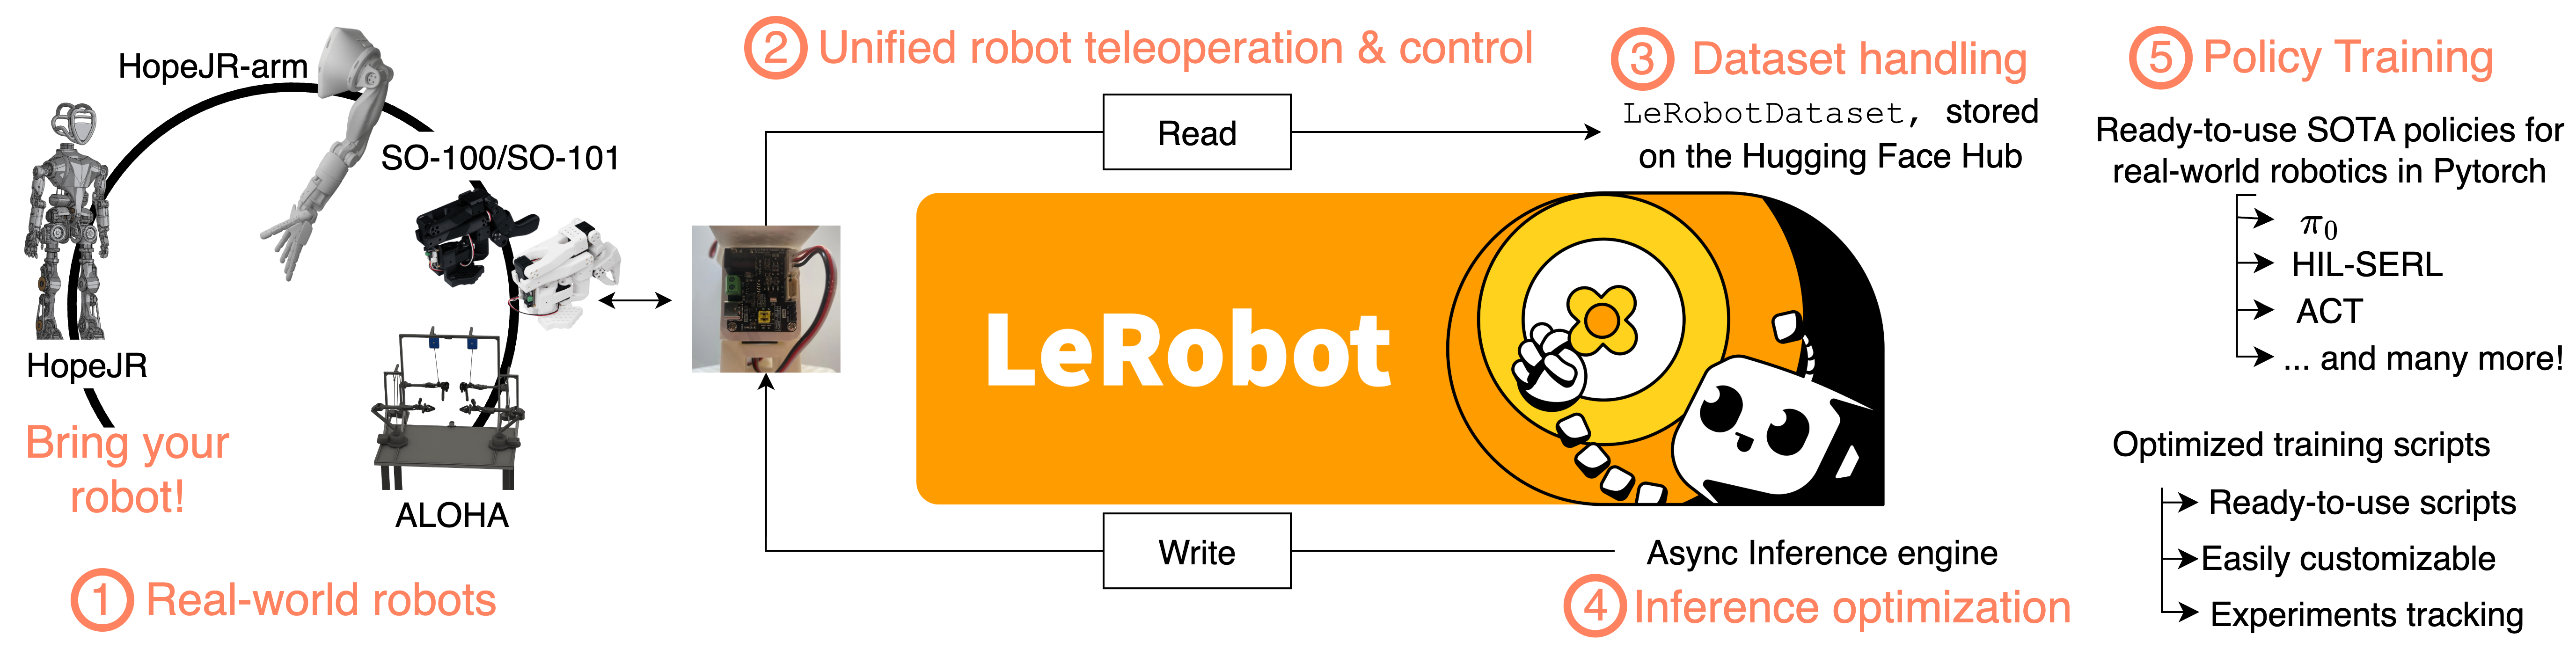
\includegraphics[width=\linewidth]{figures/ch1/ch1-lerobot-figure1.png}
    \caption{\lerobot~is the open-source library for end-to-end robotics developed by Hugging Face. The library is vertically integrated on the entire robotics stack, supporting low-level control of real-world robot devices, advanced data and inference optimizations, as well as  SOTA robot learning methods with simple implementations in pure Pytorch.}
    \label{fig:figure1}
\end{figure}

Autonomous robotics holds the premise of relieving humans from repetitive, tiring or dangerous manual tasks.
Consequently, the field of robotics has been widely studied since its first inception in the 1950s.
Lately, advancements in Machine Learning (ML) have sparked the development of a relatively new class of methods used to tackle robotics problems, leveraging large amounts of data and computation rather than human expertise and modeling skills to develop autonomous systems.

The frontier of robotics research is indeed increasingly moving away from classical model-based control paradigm, embracing the advancements made in ML, aiming to unlock (1) monolithic perception-to-action control pipelines and (2) multi-modal data-driven feature extraction strategies, together with (3) reduced reliance on precise models of the world and (4) a better positioning to benefit from the growing availability of open robotics data.
While central problems in manipulation, locomotion and whole-body control demand knowledge of rigid-body dynamics, contact modeling, planning under uncertainty, recent results seem to indicate learning can prove just as effective as explicit modeling, sparking interest in the field of \emph{robot learning}.
This interest can be largely justified considering the significant challenges related to deriving accurate models of robot-environment interactions.

Moreover, since end-to-end learning on ever-growing collections of text and image data has historically been at the core of the development of \emph{foundation models} capable of semantic reasoning across multiple modalities (images, text, audio, etc.), deriving robotics methods grounded in learning appears particularly consequential, especially as the number of openly available datasets continues to grow.

Robotics is, at its core, an inherently multidisciplinary field, requiring a wide range of expertise in both \emph{software} and \emph{hardware}.
The integration of learning-based techniques further broadens this spectrum of skills, raising the bar for both research and practical applications.
\lerobot~is an open-source library designed to integrate end-to-end with the entire robotics stack.
With a strong focus on accessible, real-world robots \highlight{(1) \lerobot~supports many, openly available, robotic platforms} for manipulation, locomotion and even whole-body control.
\lerobot also implements a \highlight{(2) unified, low-level approach to reading/writing robot configurations} to extend support for other robot platforms with relatively low effort. 
The library introduces \lerobotdataset, \highlight{(3) a native robotics dataset's format} currently being used by the community to efficiently record and share datasets.
\lerobot~also supports many state-of-the-art (SOTA) algorithms in robot learning---mainly based on Reinforcement Learning (RL) and Behavioral Cloning (BC) techniques---with efficient implementations in Pytorch, and extended support to experimentation and experiments tracking.
Lastly, \lerobot~defines a custom, optimized inference stack for robotic policies decoupling action planning from action execution, proving effective in guaranteeing more adaptability at runtime.

This tutorial serves the double purpose of providing useful references for the Science behind---and practical use of---common robot learning techniques.
To this aim, we strike to provide a rigorous yet concise overview of the core concepts behind the techniques presented, paired with practical examples of how to use such techniques concretely, with code examples in \lerobot, for researchers and practitioners interested in the field of robot learning.
This tutorial is structured as follows:
\begin{itemize}
\item Section~\ref{sec:classical} reviews classical robotics foundations, introducing the limitations of dynamics-based approaches to robotics.
\item Section~\ref{sec:learning-rl} elaborates on the limitations of dynamics-based methods, and introduce RL as a practical approach to solve robotics problems, considering its upsides and potential limitations.
\item Section~\ref{sec:learning-imitation} further describes robot learning techniques that aim at solving single-tasks learning, leveraging BC techniques to autonomously reproduce specific expert demonstrations.
\item Section~\ref{sec:learning-foundation} presents recent contributions on developing generalist models for robotics applications, by learning from large corpora of multi-task \& multi-robot data (\emph{robotics foundation models}).
% \item Lastly, Section~\ref{sec:extensions} covers emerging directions in robot learning research, introducing recent works in post-training techniques for robotics foundation models, as well as recent works in world models for robotics.
\end{itemize}

Our goal with this tutorial is to provide an intuitive explanation of the reasons various disparate ideas from Machine Learning (ML) have converged and are powering the current evolution of Robotics, driving the unprecedented progress we see today.
We complement our presentation of the most common and recent approaches in robot learning with practical code implementations using \lerobot, and start here by presenting the dataset format introduced with \lerobot.

\subsection{\lerobotdataset}

\lerobotdataset~is a standardized dataset format designed to address the specific needs of robot learning research, and it provides a unified and convenient access to robotics data across modalities, including sensorimotor readings, multiple camera feeds and teleoperation status.
\lerobotdataset~also accommodates for storing general information regarding the data being collected, including textual descriptions of the task being performed by the teleoperator, the kind of robot used, and relevant measurement specifics like the frames per second at which the recording of both image and robot state's streams are proceeding.

In this, \lerobotdataset~provides a unified interface for handling multi-modal, time-series data, and it is designed to seamlessly integrate with the PyTorch and Hugging Face ecosystems.
\lerobotdataset~can be easily extended by users and it is highly customizable by users, and it already supports openly available data coming from a variety of embodiments supported in \lerobot, ranging from manipulator platforms like the SO-100 arm and ALOHA-2 setup, to real-world humanoid arm and hands, as well as entirely simulation-based datasets, and self-driving cars.
This dataset format is built to be both efficient for training and flexible enough to accommodate the diverse data types encountered in robotics, while promoting reproducibility and ease of use for users. 

\subsubsection{The dataset class design}

A core design choice behind \lerobotdataset~is separating the underlying data storage from the user-facing API.
This allows for efficient storage while presenting the data in an intuitive, ready-to-use format.

Datasets are always organized into three main components:
\begin{itemize}
\item \textbf{Tabular Data}: Low-dimensional, high-frequency data such as joint states, and actions are stored in efficient memory-mapped files, and typically offloaded to the more mature \texttt{datasets} library by Hugging Face, providing fast with limited memory consumption.
\item \textbf{Visual Data}: To handle large volumes of camera data, frames are concatenated and encoded into MP4 files. Frames from the same episode are always grouped together into the same video, and multiple videos are grouped together by camera. To reduce stress on the file system, groups of videos for the same camera view are also broke into multiple sub-directories, after a given threshold number.
\item \textbf{Metadata} A collection of JSON files which describes the dataset's structure in terms of its metadata, serving as the relational counterpart to both the tabular and visual dimensions of data. Metadata include the different feature schema, frame rates, normalization statistics, and episode boundaries.
\end{itemize}

For scalability, and to support datasets with potentially millions of trajectories (resulting in hundreds of millions or billions of individual camera frames), we merge data from different episodes into the same high-level structure.
Concretely, this means that any given tabular collection and video will not typically contain information about one episode only, but rather a concatenation of the information available in multiple episodes.
This keeps the pressure on the file system limited, both locally and on remote storage providers like Hugging Face, though at the expense of leveraging more heavily relational-like, metadata parts of the dataset, which are used to reconstruct information such as at which position, in a given file, an episode starts or ends.
An example struture for a given \lerobotdataset~would appear as follows:
\begin{itemize}
\item \texttt{meta/info.json}: This metadata is a central metadata file. It contains the complete dataset schema, defining all features (e.g., \texttt{observation.state}, \texttt{action}), their shapes, and data types. It also stores crucial information like the dataset's frames-per-second (\texttt{fps}), \lerobot's version at the time of capture, and the path templates used to locate data and video files.
\item \texttt{meta/stats.json}: This file stores aggregated statistics (mean, std, min, max) for each feature across the entire dataset, used for data normalization for most policy models and accessible externally via \texttt{dataset.meta.stats}.
\item \texttt{meta/tasks.jsonl}: This file contains the mapping from natural language task descriptions to integer task indices, which are useful for task-conditioned policy training.
\item \texttt{meta/episodes/*} This directory contains metadata about each individual episode, such as its length, the corresponding task, and pointers to where its data is stored in the dataset's files. For scalability, this information is stored in files rather than a single large JSON file.
\item \texttt{data/*}: Contains the core frame-by-frame tabular data, using parquet files to allow for fast, memory-mapped access. To improve performance and handle large datasets, data from multiple episodes are concatenated into larger files. These files are organized into chunked subdirectories to keep the size of directories manageable. A single file typically contains data for more than one single episode.
\item \texttt{videos/*}: Contains the MP4 video files for all visual observation streams. Similar to the \texttt{data/} directory, the video footage from multiple episodes is concatenated into single MP4 files. This strategy significantly reduces the number of files in the dataset, which is more efficient for modern filesystems.
\end{itemize}

\subsection{Code Example: Batching a (Streaming) Dataset}

This section provides an overview of how to access datasets hosted on Hugging Face using the \lerobotdataset~class.
Every dataset on the Hugging Face Hub containing the three main pillars presented above (Tabular, Visual and relational Metadata), and can be assessed with a single instruction.

In practice, most reinforcement learning (RL) and behavioral cloning (BC) algorithms tend to operate on stack of observation and actions.
For the sake of brevity, we will refer to joint spaces, and camera frames with the single term of \emph{frame}.
For instance, RL algorithms may use a history of previous frames \(o_{t-H_o:t} \) to mitigate partial observability, and BC algorithms are in practice trained to regress chunks of multiple actions (\(a_{t+t+H_a} \)) rather than single controls.
To accommodate for these specifics of robot learning training, \lerobotdataset~provides a native windowing operation, whereby users can define the \emph{seconds} of a given window (before and after) around any given frame, by using the \texttt{delta\_timestemps} functionality.
Unavailable frames are opportunely padded, and a padding mask is also returned to filter out the padded frames.
Notably, this all happens within the \lerobotdataset, and is entirely transparent to higher level wrappers commonly used in training ML models such as \texttt{torch.utils.data.DataLoader}.

Conveniently, by using \lerobotdataset~with a Pytorch \texttt{DataLoader} one can automatically collate the individual sample dictionaries from the dataset into a single dictionary of batched tensors for downstream training or inference.
\lerobotdataset~also natively supports streaming mode for datasets.
Users can stream data of a large dataset hosted on the Hugging Face Hub, with a one-line change in their implementation.
Streaming datasets supports high-performance batch processing (ca. 80-100 it/s, varying on connectivity) and high levels of frames randomization, key features for practical BC algorithms which otherwise may be slow or operating on highly non-i.i.d. data.
This feature is designed to improve on accessibility so that large datasets can be processed by users without requiring large amounts of memory and storage.

\begin{pbox}[label={ex:dataset-batching}]{Batching a (Streaming) Dataset 
    %\\ \url{flow_matching/examples/standalone_discrete_flow_matching.ipynb}
}
\inputminted{python}{snippets/ch1/01_dataset.py}
\end{pbox}

\subsection{Code Example: Collecting Data}
\label{paragraph:collecting-data}

\begin{pbox}[label={ex:record_data}]{Recording Expert Data}
\inputminted{python}{snippets/ch1/02_record_data.py}
\end{pbox}

\section{Classical Robotics}

\epigraph{\textit{Know your enemy} [...]}{Sun Tzu}

\begin{tldr}
Exploring learning-based techiniques versus purely dynamics-based approaches is motivated by the interest in (1) generalizing to tasks and embodiments (2) reducing dependancy on human expertise (3) leveraging historical trends on the production of data.
\end{tldr}

\subsection{Artificial motion}
\label{sec:classical}

Robotics is concerned with producing artificial motion in the physical world in a way that is useful, reliable and safe.
Thus robotics is at its very core an inherently multidisciplinar domain: producing motion requires interfacing various hardware and software componets, each at various levels.
Defining a concept of usefulness typically depends on a profound understanding of the applicative domain considered, whereas ensuring reliable and safe execution moreso relies on estimating the inhernet uncertainty in the robot's actions, guaranteeing adaptiveness of control while optimizing for performance, and more.
Knowledge of mechanical, electrical, and software engineering, as well as rigid-body mechanics and control theory have therefore been quintessential in robotics since the field first developed.
Lately, Machine Learning (ML) has proven useful in complementing said disciplines, making usage of the robotics data currently becoming more and more available.
As a direct consequence of its multi-disciplinar nature, robotics developed as a rather wide array of methods, all concerned with the main purpose of producing artificial motion in the physical world.

Methods to produce robotics motion range from traditional \emph{explicit} models---leveraging precise descriptions of the mechanics of robots' rigid bodies and their interactions with eventual obstancles in the robots environment---to fully \emph{learning-based} systems, offloading modelling the robot mechanics and rather treating motion as a statistical pattern to learn given multiple sensorimotor readings~\citep{bekrisStateRobotMotion2024}.
Between these two extrema, a variety of methods exists, with many borrowing traits from the opposite extremum to tackle specific challenges.
On the one hand, as learning-based systems can benefit from information relative to the physics of particularly static tasks, Temporal Difference (TD) methods have been complemented with Model-Predictive Control (MPC)~\citep{hansenTemporalDifferenceLearning2022}.
On the other hand, explicit models may be relying on assumptions proving overly simplicistic---or even unrealistic---in practice, as in the case of assuming perfect observability of a robot state using sensorimotor readings. In this context, feedback loops at the control level help mitigate the effects of poor state estimation, complementing the motion planning process with discrepancy-from-target information, similarily to how loss functions are used in statistical learning.
Figure~\ref{fig:generating-motion-atlas} graphically illustrates the most relevant techniques developed for general-purpose applications. 
This categorization is far from being exhaustive, and we refer the interested reader to~\citet{bekrisStateRobotMotion2024} for a much more comprehensive overview of both general and application-specific methods for motion generation.
In this section, we aim at introducing the inherent benefit of learning-based approaches to robotics---the core focus on this tutorial---in the context of increasing availability of robot-data

\subsection{Different kinds of motion} 
% Robotics atlas: moving through and modifying an environment (and combinations). That is, (1) locomotion (2) manipulation and (3) whole-body control
At its core, robotics deals with producing motion via actuating joints connecting nearly entirely-rigid links. 
A key distinction between focus areas in robotics is based on whether the generated motion modifies (1) the relative state of the robot with respect to its environment, (2) the absolute state of the environment or (3) both relative and absolute state (Figure~\ref{fig:robotics-platforms-atlas}).
For instance, (1) may consist in changes in the robot's physical location within its environment. 
Generally, modifications to a robot's location within its environment may be considered instances of the general \emph{locomotion} problem, further specified as \emph{wheeled} or \emph{legged} locomotion based on whenever a robot makes use of wheels or leg(s) to move in the environment.
Further, (2) are typically achieved \emph{through} the robot, i.e. generating motion to cause a perform an action inducing a desirable modification, effectively manipulating (\emph{manipulation}) the environment. 
Manipulation is a well studied problem class in robotics, nowadays solved in practice for static and repetitive manipulation tasks, typically performed in controlled and precisely studied scenarios for instance via industrial robots employed at various stages of manifacturing processes.
Lastly, an increased level of dynamism in the robot-environment interactions can be obtained combining (1) and (2), thus designing systems capable to move within \emph{and} interact with their environment, falling under the category of \emph{whole-body control}, and is characterized by a typically much larger set of control variables compared to either locomotion or manipulation alone.

% Focus on learning-based approaches and manipulation
The traditional body of work developed since the very inception of robotics is increasingly more complemented by learning-based approaches.
ML has indeed proven particularly transformative across the entire robotics stack, first empowering planning-based techniques with improved state estimation used for traditional planning~\citep{tangPerceptionNavigationAutonomous2023} and then end-to-end replacing controllers, from perception to action~\citep{koberReinforcementLearningRobotics}.
Work in producing robots capable of navigating a diverse set of terrains demonstrated the premise of both dynamics and learning-based approaches for locomotion~\citep{griffinWalkingStabilizationUsing2017,jiDribbleBotDynamicLegged2023,leeLearningQuadrupedalLocomotion2020,margolisRapidLocomotionReinforcement2022}, and recent works on whole-body control indicated the premise of learning-based approaches to generate rich motion in complex robot including humanoids~\citep{zhangWoCoCoLearningWholeBody2024,nvidiaGR00TN1Open2025}.
Manipulation has also been widely studied, particularly considering its aforementioned relevance for many impactful applications ranging from high-risk applications for humans~\citep{fujitaDevelopmentRobotsNuclear2020,alizadehComprehensiveSurveySpace2024,fujitaDevelopmentRobotsNuclear2020} to manifacturing~\citep{sannemanStateIndustrialRobotics2020}.
While explicit models relying on precise descriptions of the dynamics and knowledge of the robot-environment system have been the key milestones in the development of modern robotics, recent works leveraging learning-based techniques for manipulation proved particularly promising in surpassing scalability and practical applicability challenges~\citep{koberReinforcementLearningRobotics}.
Consequently, this work is primarily focused on the application of ML to robotics (\emph{robot learning}), and is particularly \emph{focused on manipulation}.

\subsection{A Toy Example: (Planar) Manipulation}
% Full physical description by means of forward kinmeatics to generate movement
Robot manipulators typically consist of a series of links and joints, all connected to an \emph{end-effector}.
In this example, we wish to provide a concrete example of a pick-and-place task, a relatively simple manipulation task whereby a robot reaches, grasps, moves and releases an object in space through a gripper end-effector.
Links and joints are considered responsible for generating motion, while the end effector is instead used to perform specific actions at the target location (e.g., grasping/releasing objects via closing/opening a gripper, using a specialized tool like a screwdriver or any measurement device).

Recently, the development of low-cost manipulators like the Aloha~\citep{zhaoLearningFineGrainedBimanual2023} Aloha-2~\citep{aldacoALOHA2Enhanced} and SO-100/SO-101~\citep{knightStandardOpenSO100} platforms significantly lowered the barrier to entry to robot learning research, considering their accessibility compared to more traditional platforms like the Franka or Panda robot~\ref{fig:robotic-platforms-costs}. 
As a consequence, works on robot learning increasingly tackle the problem of learning to perform highly dexterous tasks using said low-end platforms: a long-standing challenge in manipulation.

Deriving an intuition as per why learning-based approaches are gaining in popularity requires briefly analyzing traditional approaches for manipulation, leveraging forward/inverse kinematics and potentially control theory to account for disturbances and misestimations.
Traditionally, manipulation combines insights from fields including spatial algebra, optimization theory, control theory, and more. 
Providing a detailed overview of these fields fall (well) beyond the scope of this tutorial, hence we refer the reader to works including~\citet{sicilianoSpringerHandbookRobotics2016, lynchModernRoboticsMechanics2017, tedrakeRoboticManipulationPerception, tedrakeUnderactuatedRoboticsAlgorithms} for a more comprehensive description of these methods.
Here, we mostly wish to highlight the main reasons why the field of robotics is increasingly moving \emph{away} from these legacy methods.

Let us consider the (simple) case where the SO-100 is restrained from actuating (1) the shoulder pane and (2) the wrist flex and roll motors. 
This effectively reduces the degrees of freedom of the SO-100 from the original 5+1 (5 actuators + end effector) to 2+1 (shoulder lift, elbow flex + gripper), yielding the planar manipulator robot presented in Figure~\ref{fig:make-so100-planar-manipulator}, where spheres represent actuators yielding and lines links from the base of the stilifyied SO-100 to its end-effector (\emph{ee}, gripper).
Further, let us make the simplifying assumptions actuators can yield rotations in the links up to \( 2 \pi \) radians with respect to a given frame of reference.
In practice, this is seldom the case due to movement obstructions caused by the robot body. 
For instance, the shoulder lift cannot produce counter-clockwise movement due to the presence of the robot's base used to secure the SO-100 to its support and host the robot bus.
These simplifying assumptions leave us with the planar manipulator of Figure~\ref{fig:planar-manipulator-free}, free of moving its end-effector by controlling the angles \( \theta_1 \) and \( \theta_2 \), jointly referred to as \emph{robot's configuration} and indicated with \( q = [\theta_1, \theta_2 ] \in [0, 2\pi]^2 \).
In this tutorial, we do not cover spatial algebra and frames of reference, and we instead refer the interested reader to \cite[Chapter~2]{lynchModernRoboticsMechanics2017|} and \cite[Chapter~3]{tedrakeRoboticManipulationPerception} for excellent explanations of mechanics and the theoretical foundations of producing motion.

Considering the (toy) example presented in Figure~\ref{fig:planar-manipulation-simple}, then we can analytically write the end-effector's position \( p \in \mathbb R^2 \) as a function of the control applied, \( p = p(q), p: \mathcal Q \mapsto \mathbb R^2 \). 
In particular, we have:
\begin{equation*}
p(q) = 
\begin{pmatrix}
p_x(\theta_1, \theta_2) \\  
p_x(\theta_1, \theta_2)
\end{pmatrix}
=
\begin{pmatrix}
l_1 \cos(\theta_1) + l_2 \cos(\theta_1 + \theta_2) \\
l_1 \sin(\theta_1) + l_2 \sin(\theta_1 + \theta_2)
\end{pmatrix}
\end{equation*}
Deriving the end-effector's \emph{pose} \( p \in \mathcal{P} \subset \mathbb{R}^{\frac{n(n+1)}{2}} \) (position and orientation) starting from the configuration \( \q in \mathcal Q \subset \mathcal R^n \) of a \( n \)-joints robot is a problem referred to as \emph{forward kinematics} (FK), whereas identifying the configuration that corresponds to a given target pose is termed \emph{inverse kinematics} (IK).
In that, FK is used to map a robot configuration into end-effector position, whereas IK is used to derive what configuration(s) results in a given end-effector pose.
In the simplified case here considered, one can solve the problem of controlling the end-effector's location to reach a goal position \( p^* \) by solving analytically for \( q: p(q) = f_{\FK}(q) = p^*\).
However, in the general case, one might not be able to solve this problem analytically, and can typically resort to iterative optimization methods comparing candidate solutions based using a loss function (in the simplest case, \( \Vert p(q) - p^* \Vert_2^2 \) is a natural candidate), yielding:

\begin{align}
\min_{q \in \mathcal Q} \Vert p(q) - p^* \Vert_2^2
\label{eq:ik_problem}
\end{align}

Analytical solutions for FK are even less appealing when one considers the presence of obstacles in the robot's workspace, resulting in constraints on the possible values of \( q \in \mathcal Q \subset [-\pi, +\pi]^n \subset \mathbb R^n \) in the general case of \(n\)-links robots.
For instance, the robot in Figure~\ref{fig:planar-manipulator-floor} is (very naturally) obstacled by the presence of the surface upon which it rests: \( \theta_1 \) can now exclusively vary within \([-\pihalf,  \pihalf] \), while possible variations in \( \theta_2 \) depend on \( \theta_1 \) (when \( \theta_1 \to \pm \pihalf  \), further downwards movements are restricted).
Even for a simplified kinematic model such as the one considered here, solving~\ref{eq:ik_problem} is in general non-trivial, particularly considering an arbitrary \( \mathcal Q \) itself may change across problems.
Figure~\ref{fig:planar-manipulation-floor-shelf} provides another such example of how analytical solutions might fail to prove effective, even in our extremely simplified settings---if an obstacle was to be positioned in the robot environment, a new set of constraints based on the position of this new obstacle would emerge, potentially resulting in unfeasibility of the problem.

Further, IK---selecting the \( q \) solving \ref{eq:ik_problem}---only proves useful in determining information regarding to the robot's configuration in the goal configuration, and crucially does not provide information on the \emph{trajectory} to follow over time to reach a target pose.
\emph{Differential} inverse kinematics (diff-IK) complements IK by enabling trajectory tracking. 
Let \( J(q) \) denote the Jacobian matrix of (partial) derivatives of the FK-function \( f_\FK \mathcal Q \mapsto \mathcal P \), \( J(q) = \frac{\partial f_{FK}(q)}{\partial q } \), then one can apply the chain rule to any \( p(q) = f_{\FK}(q) \) deriving \( \dot p = J(q) \dot q \), finally relating variations in the robot configurations to variations in positions, thus providing a platform to for control.

Thus, given a desired end-effector velocity trajectory \( \targetvel \) indicating (1) which points in space to traverse and (2) how much time to spend in each region, diff-IK finds \( \dot q(t) \) by solving a \( \lambda \)-regularized version of \ref{eq:ik_problem}, solving for \emph{velocities} instead of \emph{positions},

\begin{align}
\dot q(t) = \arg\min_\nu \; \lVert J(q(t)) \nu - \targetvel (t) \rVert_2^2
\label{eq:reg_ik_velocity}
\end{align}

Unlike control in position, \( \dot q \) is much less dependent on the environment (typically, variations in velocity are constrained by physical limits on the actuators represented with box-like constraints in \ref{eq:reg_ik_velocity}.
Conveniently, \ref{eq:reg_ik_velocity} admits the closed-form solution, \( \dot q = J(q)^+ \targetvel \), where \( J^+(q) \) denotes the Moore-Penrose pseudo-inverse of \( J(q) \).
Finally, discrete-time trajectories can then obtained using forward integration,
\[
q_{t+1} = q_t + \Delta t\,\dot q_t
\]
Following trajectories with diff-IK is a valid option in well-controlled and static environments like manipulators in industrial applications, and relies on the ability to define a set of target velocities to track \( [\targetpos_0, \targetpos_1, \dots, \targetpos_k ] \)---a task largely carried out by human experts and prone to errors.
Furthermore, diff-IK relies on the ability to (1) access \( J(q) \, \forall q \in \mathcal Q \) and (2) compute its pseudo-inverse at every iteration of a given control cycle---an assumption complicated to guarantee in highly dynamical settings or for complex instances of FK (nonlinear dynamics).

\subsubsection{Adding feedback loops}
While effective when a goal has been well specified, the performance of diff-IK can degrade significantly in the presence of modeling/tracking errors or in the presence of non-modeled dynamics in the environment.
One such case is presented in Figure~\ref{fig:planar-manipulator-box-velocity}, where another rigib body is moving in the environment with velocity \( \dot x_B \). 
Accounting analytically for the presence of this disturbance---for instance, to prevent \( l_1 \) from ever colliding with the object---requires access to \( \dot x_B \) and of a reference position \( x_{B,0} \) for the object \( B \), to derive the equation characterizing its motion.
For less predictable disturbances (e.g., \( \dot x_B \leftarrow x_B + \eps, \eps \sim N(0,1) \) one could attain similar results by adding a condition on the distance between the midpoint of \( l_1 \) and \( x_B \), enforced through a feedback loop on the position of the robot and object at each control cycle.

To mitigate the effect of modeling errors, sensing noise and other disturbances, classical pipelines augment diff-IK with feedback control on the measured error between the target position and the one measured, \( \Delta p = \targetpos - p(q) \), hereby modifying the control applied to \( \dot q = J(q)^+ (\targetvel + \lambda \Delta p \), with \( \lambda \) defined as the gain.
More advanced techniques for control consisting in feedback linearization, PID control, or LQR/MPC can also be employed to stabilize tracking and reject moderate perturbations (\cite[Chapter~8]{sicilianoSpringerHandbookRobotics2016}, or \cite[Chapter~8]{tedrakeRoboticManipulationPerception} for a simplified example in the case of a point-mass system).
Nonetheless, tuning gains remains laborious and system-specific: In manipulation, intermittent contacts induce hybrid dynamics (mode switches) and discontinuities in the effective Jacobian, challenging stability guarantees and often necessitating conservative gains and substantial hand-tuning.

We point the interested reader to \cite[Chapter~2,7,8]{sicilianoSpringerHandbookRobotics2016}, \cite[Chapter~6,11]{lynchModernRoboticsMechanics2017}, and \cite[Chapter~3,8]{tedrakeRoboticManipulationPerception} for extended coverage of FK, IK and diff-IK and control for (diff-)IK.

\subsection{Limitations}
Depiste the last 60+ years of robotics research, autonomous robots are still largely incapable of performing tasks at human-level performance in the physical world across (1) robot embodiments (different manipulators, different locomotion platforms, etc.) and (2) tasks (tying shoe-laces, manipulating a diverse set of objects).
While essential in the early development of robotics, the aforementioned methods require significant human expertise to be used in practice, and are typically specific to a particular applicative problem. We argue this follows from various reasons.

Robotics pipelines have been \highlight{developed sequentially, hand-engineering the different block architectures} for specific purposes. 
Sensing, state estimation, mapping, planning, (diff-)IK, and low-level control have been traditionally developed as distinct modules with fixed interfaces.
Pipelining these highly specific modules is a error-prone, and brittleness emerges whenever shifts with respect to a considered pipeline incur (e.g., changes in lighting for sensing, occlusion/failure of sensors).
Adapting such a stack to new tasks or embodiments often entails re-specifying objectives, constraints, and heuristics at multiple stages, incurring significant engineering overhead.

Classical planners operate on compact, assumed-sufficient state representations; extending them to reason directly over raw, heterogeneous and noisy data streams is non-trivial.
This results in a \highlight{limited scalability to multimodal data and multitask settings}, as incorporating high-dimensional perceptual inputs (RGB, depth, tactile, audio) traditionally required extensive engineering efforts to extract meaningful efforts for control. 
Moreover, the large number of tasks, coupled with the adoption of \emph{per-task} planners, goal parameterizations, and safety constraints, results in an explosion in design and validation effort, with little opportunity to share experience across tasks.

Further, even setting aside integration and scalability challenges, developing accurate modeling of contact, friction, and compliance for complicated remains difficult.
Rigid-body approximations are often insufficient in the presence of deformable objects, and \highlight{relying on approximated models hinders real-world applicability}.
In the case of complex and/or non-linear dynamics, even moderate mismatches in contact parameters, unmodeled flexibilities, or grasp-induced couplings can qualitatively affect the observed dynamics, degrading the reliability of  the model obtained.
Even a perfect model of reality would need to relax the stationarity assumptions that are typically made in control. Explicitly modeling the effects of payload changes, tool substitutions, temperature-dependent friction, and component-aging on the resulting dynamics is, in most cases, simply unfeasible.

Lastly, dynamics-based methods (naturally) overlook the rather recent phenomenon of the \highlight{explosion of openly-available robotics data}, following a similar pattern to the explosion of image and text data.
The curation of academic datasets by large centralized groups of human experts in robotics~\citep{OpenXEmbodimentRobotic,DROIDLargeScaleIntheWild,agibot-world-contributorsAgiBotWorldColosseo2025} is now increasingly complemented by a \highlight{growing number of robotics datasets contributed in a decentralized fashion} by individuals with varying expertises (Figure~\ref{fig:lerobot_datasets_trend}).
If not tangentially, dynamics-based approaches are not posed to maximally benefit from this new trend, holding the premise of allowing generalization in the space of tasks and embodiments, like data was the cornerstone for advancements in vision~\citep{alayracFlamingoVisualLanguage2022} and natural-language understanding~\citep{openaiGPT4TechnicalReport2024}.

Taken together, these limitations motivate the exploration of learning-based approaches that can (1) integrate perception and control more tightly, (2) adapt across tasks and embodiments with reduced expert intervention and (3) scale gracefully in performance as more robotics data becomes available.
\epigraph{\textit{The best material model for a cat is another, or preferably the same cat}}{Norbert Wiener}

\section{Robot Learning}
\label{sec:learning}

Learning-based techniques for robotics naturally address the limitations presented in~\ref{sec:classical} (Figure~\ref{fig:robot-learning-upsides}).
Learning-based techniques typically rely on prediction-to-action (\emph{visuomotor policies}), thereby directly mapping sensorimotor inputs to predicted actions, streamlining the harmonization of control policies.
Mapping sensorimotor inputs to actions directly also allows to add diverse input modalities over time, leveraging the automatic feature extraction characteristic of most common learning systems.
Further, learning-based approaches can in principle entirely bypass modeling efforts and instead rely exclusively on interactions data, proving transformative when dynamics are challenging to model or unknown.
Lastly, we argue learning for robotics (\emph{robot learning}) is naturally well posed to leverage the growing amount of robotics data openly available, just as computer vision first and natural language processing later did historically benefit from large scale corpora of (possibly non curated) data.
As it largely leverages techniques and results developed within more mature subfields within ML (computer vision-based feature extractors, language-based semantics, etc.), robot learning is thus posed to potentially benefit from the growing amount of motion data available, in great part overlooked by dynamics-based approaches.

Robot learning is a field at its relative nascent stages, and no prevalent technique(s) proved distinctly better than others.
Still, two major classes of methods gained prominence in applications of ML to robotics: \highlight{reinforcement learning (RL)} and \highlight{behavioral cloning (BC)}.
In this section, we provide a conceptual overview of applications of the former to robotics, as well as introduce practical examples of how to use RL within \lerobot.
We then introduce the major limitations RL suffers from, introducing BC shortly after.
Importantly, (Figure~\ref{fig:robot-learning-atlas}) we decided to include generalist robot models~\citep{blackpi0VisionLanguageActionFlow2024,shukorSmolVLAVisionLanguageActionModel2025} alongside task-specific BC methods.
While very different in spirit---generalist models learn to take instructions as input and to use them to generate motion valid across many tasks---foundation models like \( \pi_0 \), for instance, are largely trained to reproduce trajectories contained in a large training set of input demonstrations.
This distinction being made, we argue generalist policies can indeed be grouped alongside other BC methods.

Figure~\ref{fig:robot-learning-atlas} illustrates this classification graphically, explicitly listing all the robot learning policies currently available in \lerobot: Action Chunking with Transformers (ACT)~\citep{zhaoLearningFineGrainedBimanual2023}, Diffusion Policy~\citep{chiDiffusionPolicyVisuomotor2024}, Vector-Quantized Behavior Transformer (VQ-BeT)~\citep{leeBehaviorGenerationLatent2024}, \( \pi_0 \)~\citep{black$p_0$VisionLanguageActionFlow2024}, SmolVLA~\citep{shukorSmolVLAVisionLanguageActionModel2025}, Human-in-the-loop Sample-efficient RL (HIL-SERL)~\citep{luoPreciseDexterousRobotic2024} and TD-MPC~\citep{hansenTemporalDifferenceLearning2022}.

\subsection{RL for Robotics}
Applications of RL to robotics have been long studied, to the point the relationship between these two disciplines has been compared to that between physics and matematics~\citep{koberReinforcementLearningRobotics}.
Indeed, due to their interactive and sequential nature, many robotics problems can be directly mapped to RL problems.
Figure~\ref{fig:robotics-with-rl-examples} depicts two of such cases. Manipulating a tiling belt into its correct position is a sequential problem where at each cycle the controller needs to adjust the position of the robotic arms based on their current configuration and the state of the tiling belt. 
In this example, sequentiality arises from the impossibility of placing the belt in its goal position right away from any starting position.
Figure~\ref{fig:robotics-with-rl-examples} also shows an example of a locomotion problem, where sequentiality is inherent in the problem formulation. Sliding to the side, the controller has to constantly keeps adjusting to the robot's propioperception, avoiding failure (falling).

\subsubsection{A (Concise) Introduction to RL}
The RL framework~\citep{suttonReinforcementLearningIntroduction2018}, which we briefly introduce here, has often been used to model robotics problems~\citep{koberReinforcementLearningRobotics}.
RL is a subfield within ML fundamentally concerned with the development of autonomous systems (\emph{agents}) learning how to \emph{continuously behave} in an evolving environment, developing control \emph{policies} to better act when in a given situation.
Crucially for robotics, agents improve via trial-and-error only, entirely bypassing the need to develop explicit models of the problem dynamics, and rather exploiting interaction data only.
In RL, this feedback loop between actions and outcomes is established through the agent sensing a scalar quantity (\emph{reward}, Figure~\ref{fig:rl-most-famous-pic}).

Formally, interactions between an agent and its environment are typically modeled via a Markov Decision Process (MDP).
Representing robotics problems via MDPs offers several advantages, including (1) incorporating uncertainty through MDP's inherently stochastic nature and (2) providing a theoretically sound framework for learning without an explicit dynamic model.
While accommodating also a continuous time formulation, MDPs are typically considered in discrete time in RL, considering interactions to atomically take place over the course of discrete \emph{timestep} \( t=0,1,2,3, \dots, T \).
MDPs allowing for an unbounded number of interactions ( \( T \to + \infty \) ) are typically termed \emph{infinite-horizon}, and opposed to \emph{finite-horizon} MDPs in which \( T \) cannot grow unbounded.
Unless diversely specified, we will only be referring to discrete-time episodic MDPs.


Formally, a Markov Decision Process (MDP) is a tuple \( \mathcal M = (\statespace, \actionspace, \dynamics, r, \gamma, \rho) \), where:
\begin{itemize}
    \item \(\statespace\) is the \emph{state space}; \(\state \in \statespace\) denotes the (possibly non-directly observable) environment state at time \(t\). In robotics, states often comprise robot configuration and velocities (\(q_t, \dot q_t\)), and can accomodate sensor readings such as camera or audio streams.
    \item \(\actionspace\) is the \emph{action space}; \(\action \in \actionspace\) may represent joint torques, joint velocities, or even end-effector commands. In general, actions correspond to commands intervenings on the configuration of the robot. 
    \item \(\dynamics\) represents the (possibly non-deterministic) environment dynamics, with \(\dynamics: \statespace \times \actionspace \times \statespace \mapsto [0, 1] \) corresponding to \( \dynamics \, \transition = \transitionprob \). For instance, for a planar manipulator dynamics can typically be considered deterministic when the environment is fully described (Figure~\ref{fig:planar-manipulation-simple}), and stochastic when disturbances depending on non-observable parameters intervene (Figure~\ref{fig:planar-manipulator-box-velocity}).
    \item \(r: \statespace \times \actionspace \times \statespace \to \mathbb R\) is the \emph{reward function}, weighing \( \transition \) in the context of an arbitrary goal. For instance, a simple reward function for quickly moving the along the \( x \) axis in 3D-space could be based on the position of the robot along the \( x \) axis~(\(p_x\)), present negative penalties for falling over (measured from \( p_z \)) and a introduce bonuses \( \dot p_x \) for speed.
\end{itemize}
Lastly, \(\gamma \in [0,1)\) represent the discount factor regulating preference for immediate versus long-term reward (with a horizon of \( \tfrac{1}{1-\gamma} \)), and \( \rho \) is the distribution defined over \(\statespace, \) to sample the initial state, \( s_0 \sim \rho \).

For MDPs, a \emph{trajectory} of length \(T\) is the (random) sequence
\begin{equation}\label{eq:trajectory_definition}
    \tau = \trajectory,
\end{equation}
with per-step rewards defined as \(r_t = r \transition \) for ease of notation.

Interestingly, assuming both the environment dynamics and conditional distribution over actions given states---termed \emph{policy}---to be \emph{Markovian}:
%
\begin{align}
\mathbb P(\stateplusone \vert s_t, a_t, s_{t-1}, a_{t-1}, \dots s_0, a_0 ) &= \mathbb P \transitiongiven \label{eq:dynamics_markovian} \\
\mathbb P(\action \vert \state, a_{t-1}, s_{t-1}, s_0, a_0) &= \mathbb P(\action \vert \state) \label{eq:policy_markovian}
\end{align}
%
The probability of observing a given trajectory \( \tau \) can be piece-wise factorized into
\begin{equation}\label{eq:traj_prob}
    \mathbb P(\tau) = \mathbb P (s_0) \prod_{t=0}^{T-1} \mathbb P \transitiongiven \ \mathbb P(\action \vert \state).
\end{equation}

Policies \( \mathbb P(\action \vert \state) \) are typically indicated as \( \pi(\action \vert \state) \), and often parametrized via \( \theta \), yielding \( \pi_\theta (\action \vert \state )\).
Thus, one can define the (discounted) \emph{return} associated to \( \tau \) as the (random) sum of the reward measured over it,
\[
    G(\tau) = \sum_{t=0}^{T-1} \gamma^{t} r_t
\]
Control agents seek to learn strategies (policies, \( \pi_\theta \)) maximizing the expected return \( \mathbb E G(\tau) \). 
For a given dynamics \( \mathcal D \)---i.e., for a given problem---taking the expectation over the (possibly random) trajectories resulting from acting according to a certain policy provides a direct, goal-conditioned ordering of all the possible policies obtained, yielding the (maximization) target \( J : \Pi \mapsto \mathbb R \)
\begin{align}
    J(\pi_\theta) &= \mathbb E_{\tau \sim \mathbb P_{\theta; \mathcal D}} \left[ G(\tau) \right], \label{eq:RL-j-function} \\
    \mathbb P_{\theta; \mathcal D} (\tau) &= \rho \prod_{t=0}^{T-1} \mathbb \mathcal D \transition \ \pi_\theta (\action \vert \state).\label{eq:traj-probabilities-for-policies}
\end{align}

MDPs thus naturally provide a framework to optimize over the space of the possible behaviors an agent might enact (\( \pi \in \Pi \)), searching for the \emph{optimal policy} \( \pi^* = \arg \max_{\theta} J(\pi_\theta) \).
A variety of methods have been developed in RL as standalone attemps to find (approximate) solutions to the problem of maximizing cumulative reward (Figure~\ref{fig:rl-algos-atlas}.
Popular approaches to continuous state and action space---such as those studied within robotics---include~\citet{schulmanTrustRegionPolicy2017, schulmanProximalPolicyOptimization2017, haarnojaSoftActorCriticOffPolicy2018}.
Across manipulation~\citep{openaiSolvingRubiksCube2019} and locomotion~\citep{leeLearningQuadrupedalLocomotion2020} tasks, RL proved very effective in providing a platform to (1) adopt a unified, streamlined perception-to-action pipeline, (2) natively integrate propioperception with multi-modal high-dimensional streams, learning data-driven pre-processing pipelines, (3) disregard a description of the environment dynamics, by focusing on observed interaction data rather than modeling, and (4) anchor policies in the experience collected in offline datasets.
For a more complete survey of applications of RL to robotics, we refer the reader to~\citet{koberReinforcementLearningRobotics,tangDeepReinforcementLearning2025a}.

\subsubsection{Real-world RL for Robotics}
Streamlined end-to-end control pipelines, data-driven feature extraction and a disregard of explicit modeling in favor of interaction data are all features of RL for robotics.
However, in the context of real-world robotics \highlight{RL suffers from limitations concerning machine safety and learning efficiency}.

RL explore erratically, which makes learning at the beginning dangerous for the hardware considered
Also, even the most sample efficient RL methods needs thousands of samples to learn to perform tasks from scratch. Further, accommodating for the RL setup is non trivial learning directly on the real robot because of challenges with ensuring reset etc.
So people have studied learning in simulation. This resolves issues with safety inherently, and improves on the practical aspects of using RL because many samples in simulation are attainable in a fraction of the time compared to real-world training. 
But simulation is different from the real world, and transferability problems arise.
People tried strategies including randomizing simulators to induce robustness to domain changes, or use real-world data to align simulations with the end result.
However simulators are also complex to build, and as a result using RL in real-world is still challenging.

\subsubsection{RL in \lerobot: data-driven, sample-efficient, and with human in-the-loop}
Recent work proposed leveraging for RL in the real-world using HIL-SERL

HIL-SERL is ...
HIL-SERL addresses ...
HIL-SERL works by ...
HIL-SERL presents limitations ...

\subsubsection{Code Example: Training RL Policies with \lerobot}
Outside of simulation environments, lerobot implements SERL

coding example of how HIL-SERL works

\subsubsection{Limitations of RL in Real-World Robotics: Simulators and Reward Design}
simulators for dexterous tasks are complex to build. Also, soft materials are very hard to model
reward design is also increasingly complex to derive for practical problem, and it is a big source of brittleness

\section{Robot (Imitation) Learning}
\label{sec:learning-bc-single}

\epigraph{\emph{The best material model for a cat is another, or preferably the same cat}}{Norbert Wiener}

Learning from human demonstrations provides a pragmatic alternative to the reinforcement-learning pipeline discussed in Section~\ref{sec:learning-rl}.
In real-world robotics, online exploration is typically \highlight{costly and potentially unsafe}, and (dense) reward design is \highlight{brittle and task-specific}.
In general, success detection often may require bespoke instrumentation, and episodic training demands reliable resets---all factors that complicate training RL algorithms on hardware at scale.
Behavioral Cloning (BC) sidesteps these constraints by casting control an imitation learning problem, leveraging previously collected expert demonstrations.
In this way, the objectives, preferences, and success criteria are implicitly encoded in the data, obviating hand-crafted reward shaping and reducing early-stage exploratory failures.

Formally, let \( \mathcal D = \{ \tau^{(i)} \}_{i=1}^N \) be a set of expert trajectories, with \( \tau^{(i)} = \{(o_t^{(i)}, a_t^{(i)})\}_{t=0}^{T_i} \), where \(o_t \in \obsspace \) denotes observations (e.g., images and proprioception), and \(a_t \in \actionspace \) the expert actions.
Figure~\ref{fig:ch4-bc-trajectories} shows observations over sample trajectories for a dataset collected by a human demonstrating a manipulation task on the SO-100 arm, while Figure~\ref{fig:ch4-observation-action-mapping} shows \( (o_t, a_t) \)-pairs for the same dataset, with the actions commanded by the human expert illustrated alongside the corresponding observation.
Note that differently from Section~\ref{sec:learning-rl}, in this context \( \mathcal D \) indicates an offline dataset (and not the dynamics), collecting \( N \) length-\( T_i \) \emph{reward-free} (expert) human trajectories \( \tau^{(i)} \) (and not the a trajectory for a given MDP).
In principle, (expert) trajectories \( \tau^{(i)} \) can have different lengths since demonstrations might exhibit multi-modal strategies to attain the same goal, resulting in possibly multiple, different behaviors.

Behavioral Cloning (BC)~\citep{pomerleauALVINNAutonomousLand1988a} aims at synthetizing these behaviors learning the mapping from observations to actions, and in its simplest formulation can be effectively be tackled as a \emph{supevised} learning problem, where one learns a mapping \( a_t = \mu(o_t) \) by solving
\begin{equation}\label{eq:loss-minimization-SL}
    \min_{\mu} \mathbb{E}_{(o_t, a_t) \sim \mathcal{D}^*} \mathcal L(a_t, \mu(o_t)),
\end{equation}
for a given risk function \( \mathcal L:  \mathcal A \times \mathcal A \mapsto \mathbb{R}, \ \mathcal L (a, a^\prime) \).

The expert's joint observation-action distribution \( \mathcal D^* \) is typically assumed to be unknown, similarily to a typical Supervised Learning (SL) framework\footnote{Throughout, we will adopt terminology and notation for SL in keeping with \citet{shalev-shwartzUnderstandingMachineLearning2014}}.
However, differently from standard SL's assumptions, the samples collected in \( \mathcal D \) are \emph{not} typically i.i.d., as expert demonstrations are collected \emph{sequentially} in trajectories.
In practice, this aspect can be partially mitigated by considering pairs in a non-sequential order---\emph{shuffling} the samples in \(\mathcal D \)---so that the expected risk under \( \mathcal D^* \) can be estimated using MC estimates, drawing \((o_t, a_t)\) from \( \mathcal D \), although estimates can in general be less accurate.
Another strategy to mitigate the impact of having non-i.i.d. samples relies on the possibility of interleaving BC and data collection~\citep{rossReductionImitationLearning2011}. 
However, because we consider the case where a single offline dataset \( \mathcal D \) dataset of (expert) trajectories has been entirely collected already, this more advanced method is typically not applicable to the considered setup.

Despite challenges, the BC formulation affords several operational advantages in robotics.
First, training happens offline and typically uses expert human demonstration data, hereby severily limiting risks.
Second, reward design is unnecessary in BC, as demonstrations already reflect human intent and task completion, mitigating misalignment and the risk of specification gaming (\emph{reward hacking}) otherwise inherent in purely reward-based RL~\citep{heessEmergenceLocomotionBehaviours2017}.
Third, because expert trajectories encode terminal conditions, success detection and resets are implicit in the dataset.
Finally, BC scales naturally with growing corpora of demonstrations collected across tasks, embodiments, and environments.
Crucially, BC can in principle only learn behaviors that are, at most, as good as the one exhibited by the demonstrator.
While problematic in sequential-decision making problems for which expert demonstrations are not generally available---data migth be expensive to collect, or human performance inherently suboptimal---many application of robotics benefit from relative cheap pipelines to acquire high-quality trajectories generated by humans. 

However, point-estimate policies \( \mu : \obsspace \mapsto \actionspace \) learned by solving \ref{eq:loss-minimization-SL} have been observed to suffer from (1) compounding errors~\citep{rossReductionImitationLearning2011} and (2) poor fit to multimodal distributions~\citep{florenceImplicitBehavioralCloning2022, keGraspingChopsticksCombating2020} (Figure~\ref{fig:ch4-issues-with-bc}).
Besides sequentiality in \( \mathcal D \), compounding errors are due to \emph{covariate shift}, whereby even small \( \epsilon \)-prediction errors \( 0 < \Vert \mu(o_t) - a_t \Vert \leq \epsilon \) can quickly drive the policy into out-of-distribution states, incuring in less confident generations and thus errors compounding (Figure~\ref{fig:ch4-issues-with-bc}, left).
Further, point-estimate policies typically fail to learn \emph{multimodal} (in the stastical sense) targets, common in robotics problems where multiple trajectories can be equally as good towards the realization of a given objective (e.g.,  symmetric grasps, Figure~\ref{fig:ch4-issues-with-bc}, left). 
In particular, unimodal regressors tend to average across modes, yielding indecisive or even unsafe commands~\citep{florenceImplicitBehavioralCloning2022}.
To address poor multimodal fitting,~\citet{florenceImplicitBehavioralCloning2022} propose learning the generative model \( p(o, a) \) underlying the samples in \( \mathcal D \), rather than an explicit prediction function \( \mu(o) = a \).

\subsection{A (Concise) Introduction to Generative Models}
% Generative Modeling
Generative Models (GMs) aims to learn the (stochastic) process underlying the very generation of the data collected, and it typically does so by fitting a probability distribution that approximates the unknown \emph{data distribution}, \( \mathcal D^* \).
In the case of BC, this unknown data distribution \( \mathcal D^* \) represents the expert's joint distribution over \( (o, a) \)-pairs, where \( (o,a) \sim \mathcal D^* \).
Thus, given a finite set of \( N \) pairs \(\mathcal D = \{ (o,a)_i \}_{i=0}^N\) used as an imitation learning target, GM seeks to learn a \emph{parametric} distribution \( p_\theta(o,a) \) such that (1) samples \( (o,a) \sim p_\theta(\bullet) \) resemble the input data \( \mathcal D \), and (2) high likelihood is assigned to observed regions of the unobservable \( p \).
Likelihood-based learning provides a principled training objective to achieve both objectives, and it is thus extensively used in GM~\citep{prince2023understanding}.

% VAEs
\paragraph{Variational Auto-Encoders}
A common inductive bias used in GM posits samples \( (o,a) \) arise from an unobservable latent variable \( z \in Z \), resulting in
\begin{equation}\label{eq:BC-latent-variable}
    p (o,a) = \int_{\supp{Z}} p(o,a \vert z) p(z)
\end{equation}
Intuitively, in the case of observation-action pairs \( (o, a) \), \( z \) could perhaps contain some sort of representation of the underlying task being performed by the human demonstrator.
In such case, treating \( p(o,a) \) as a marginalization over \( \supp{Z} \) of the complete joint distribution \( p(o,a,z) \) natively captures the effect different tasks have on observation-action pairs.
Figure~\ref{fig:ch4-task-effect-on-pairs} graphically illustrates this concept in the case of a (A) picking and (B) pushing task, for which, nearing the target object, the likelihood of actions resulting in opening the gripper---the higher \( q_6 \), the wider the gripper's opening---should intuitively be (A) high or (B) low, depending on the task performed.
While the latent space \( Z \) typically has a much richer structure than the set of all actual tasks performed,~\ref{eq:BC-latent-variable} still provides a solid framework to learn joint distribution conditioned on unobservable yet relevant factors.
Figure~\ref{fig:ch4-latent-variable-model} represents this framework of latent-variable for a robotics application: the true, \( z \)-conditioned generative process on assigns \emph{likelihood} \( p_\theta(\bullet \vert z) \) to the single \( (o,a) \)-pair, for a given parametric distribution \(p_\theta \) (e.g., Gaussian).
Using Bayes' theorem, we could even reconstruct the \emph{posterior} distribution on \( \supp{Z} \), \( p_\theta(z \vert o,a) \) from the likelihood \( p_\theta(o,a \vert z) \), \emph{prior} \( p_\theta(z) \) and \emph{evidence} \( p_\theta(o,a) \).

By a similar argument, given a dataset \( \mathcal D \) consisting of \( N \) i.i.d. observation-action pairs, the log-likelihood of all datapoints under \( \theta \) (in Bayesian terms, the \emph{evidence} \( p_\theta(\mathcal D)\)) can be written as:
\begin{align}
    \log p_\theta(\mathcal D) &= \log \sum_{i=0}^N p_\theta ((o,a)_i) \label{eq:evidence-definition-1}\\
                              &= \log \sum_{i=0}^N \int_{\supp{Z}} p_\theta((o,a)_i \vert z) p(z) \label{eq:evidence-definition-2}\\
                              &= \log \sum_{i=0}^N \int_{\supp{Z}} \frac{p_\theta(z \vert (o,a)_i)}{p_\theta(z \vert (o,a)_i)} \cdot p_\theta((o,a)_i \vert z) p(z) \label{eq:evidence-definition-3}\\
                              &= \log \sum_{i=0}^N \mathbb E_{z \sim p_\theta(\bullet \vert (o,a)_i)} \left[ \frac{p(z)}{p_\theta(z \vert (o,a)_i)} \cdot p_\theta((o,a)_i \vert z) \right], \label{eq:evidence-definition}
\end{align}
where we used~\ref{eq:BC-latent-variable} in~\ref{eq:evidence-definition-1}, multiplied by \(1 = \frac{p_\theta(z \vert (o,a)_i)}{p_\theta(z \vert (o,a)_i)} \) in~\ref{eq:evidence-definition-2}, and used the definition of expected value in~\ref{eq:evidence-definition}.

In the special case where one assumes distributions to be tractable, \( p_\theta (\mathcal D) \) is typically tractable too, and \(\max_\theta \log p_\theta(\mathcal D) \) provides a natural target for (point-wise) infering the unknown parameters \( \theta \) of the generative model.
Unfortunately, tractability of~\ref{eq:evidence-definition} is rarely induced by using distributions \( p \) modeled using approximators, like neural networks, to model high-dimensional, unstructured data.

In their seminal work on Variational Auto-Encoders (VAEs),~\citet{kingmaAutoEncodingVariationalBayes2022} propose two major contributions to learn complex latent-variable GMs on unstructured data: (1) propose a tractable, variational lower-bound to \ref{eq:evidence-definition} as an optimization target to learn \( \Phi \) and (2) use high-capacity function approximators to model the likelihood \(p_\theta(o,a\vert z)\) and (approximate) posterior distribution \( q_\phi(z \vert o,a) \approx p_\theta(z \vert o,a) \).

In particular, the lower bound on~\ref{eq:evidence-definition} (Evidence LOwer Bound, \emph{ELBO}) can be derived applying Jensen's inequality---\(\log \mathbb{E}[\bullet] \geq \mathbb{E} [\log (\bullet)] \)---to~\ref{eq:evidence-definition}, yielding:
\begin{align}
    \log p_\theta(\mathcal D) &\geq \sum_{i=0}^{N} \left(
            \mathbb{E}_{z \sim p_\theta(\cdot \vert (o,a)_i)} \big[ \log p_\theta((o,a)_i \vert z) \big]
            + \mathbb{E}_{z \sim p_\theta(\cdot \vert (o,a)_i)} \left[ \log \left( \frac{p(z)}{p_\theta(z \vert (o,a)_i)} \right) \right]
        \right) \\
        &= \sum_{i=0}^{N} \left(
            \mathbb{E}_{z \sim p_\theta(\cdot \vert (o,a)_i)} \big[ \log p_\theta((o,a)_i \vert z) \big]
        - \DKL \big[ p_\theta(z \vert (o,a)_i) \Vert p(z) \big]
        \right) \label{eq:ELBO-intractable}
\end{align}
The true, generally intractable posterior \( p_\theta (z \ vert o,a) \) prevents computing both the expectation and KL divergence terms in~\ref{eq:ELBO-intractable}.
Crucially,~\citet{kingmaAutoEncodingVariationalBayes2022} propose deriving the ELBO using an \emph{approximate} posterior \( q_\phi(z \vert o,a) \), resulting in the final, tractable ELBO objective,
\begin{align}
\text{ELBO}_{\mathcal D}(\theta, \phi) = \sum_{i=0}^{N} \left(
            \mathbb{E}_{z \sim q_\phi(\cdot \vert (o,a)_i)} \big[ \log p_\theta((o,a)_i \vert z) \big]
        - \DKL \big[ q_\phi(z \vert (o,a)_i) \Vert p(z) \big]
        \right)
        \label{eq:ELBO}
\end{align}
From Jensen's inequality, maximizing ELBO results in maximizing the log-likelihood of the data too, thus providing a natural, tractable optimization target.
Indeed, expectations can be estimated using MC estimates from the learned distributions in~\ref{eq:ELBO}, while the KL-divergence term can typically be computed in closed-form (1) modeling  \( \) and (2) 
A particularly intuitive explanation of learning GMs optimizing ELBO can be given considering minimizing the \emph{negative ELBO}, i.e. \( \min_{\theta, \phi} - \text{ELBO}_{\mathcal D}(\theta, \phi) = \min_{\theta, \phi}\mathbf{L^{\text{rec}}}(\theta) + \mathbf{L^{\text{reg}}}(\phi) \).

For any given \((o,a) \) pair, the expected value term of~\ref{eq:ELBO} is typically computed via MC estimates, resulting in
\[ 
-\mathbb{E}_{z \sim q_\phi(\bullet \vert o,a)} \big[ \log p_\theta(o,a \vert z) \big] = \mathbf{L^{\text{rec}}} \approx - \frac{1}{n} \sum_{i=0}^n \log p_\theta(o,a \vert z_i).
\]
Assuming \( p_\theta(o,a \vert z) \) is parametrized as an isotropic Gaussian distribution with mean \(\mu_\theta (z) \in \mathbb R^d \) and variance \( \sigma^2 \), the log-likelihood simplifies to:
\[
\log p(o,a \vert z_i) = -\frac{1}{2\sigma^{2}} \big \Vert (o,a)-\mu_\theta(z_i) \big\Vert_2^2 -\frac{d}{2}\log(2\pi \sigma^{2}) \implies \mathbf{L^\text{rec}} \approx \frac {1}{n} \sum_{i=0}^n \big\Vert (o,a) - \mu_\theta(z_i) \big \Vert^2_2
\]
In practice, samples from the learned likelihood \( p_\theta(o,a \vert z) \) are often collected drawing from parametric distributions (e.g. Gaussians) parametrized by some vector of coefficients derived from \(\mu_\theta (z), \ z \sim p_Z (\bullet) \).
In such cases, learning a GM partly corresponds to \emph{reconstructing} the examples in \( \mathcal D \), by minimizing the L2-error---a very common \emph{supervised learning} objective for continuous targets.
Further, the second term in \( -\text{ELBO}_\mathcal D(\theta, \phi) \)---\( \mathbf{\mathbf{L^{\text{reg}}}(\phi)} \)---results in the regularization of the approximate posterior, under the common modeling choice \( p(z) \sim N(\mathbf{0}, \mathbf{I}) \), which limits the expressivity of \( q_\phi(z\vert o,a) \).

% Diffusion
\paragraph{Diffusion Models}
VAEs approximate probability distributions via a \emph{single} latent variable model, assuming the underlying unknown distribution samples are obtained from can be factored according to~\ref{eq:BC-latent-variable}, and solve the variational inference problem of jointly learning the likelihood \( p_\theta \) and (approximate) posterior \( q_\phi \) for such model.
In that, the unknown data distribution \( p(o,a) \) is effectively approximated via \( \int_Z p(z) p_\theta(o,a \vert z) \), and the underlying generative process reproduced by (1) sampling a latent variable and (2) learning to decode it into a (ideally) high-likelihood sample under the (unknown) \( p(o,a) \).
Diffusion Models (DMs)~\citep{hoDenoisingDiffusionProbabilistic2020} are another class of GMs which treat the similar problem of approximating an underlying unknown data distribution---\emph{variational inference}---by partially extending VAEs to the case where \emph{multiple} latent variables influence each other and the generative process underlying \(o,a\) itself.
In particular, DMs posit the generative process can be decomposed to a series of piece-wise (Markovian) interactions between (latent) variables (Figure~\ref{fig:ch4-diffusion}), resulting in
\begin{align}
    p(\underbrace{o,a}_{= z_0}) &= \int_{\supp{Z_0}} \int_{\supp{Z_1}} \hdots \int_{\supp{Z_T}} p(z_0, z_1, \dots z_T) \label{eq:BC-multi-latent-model-1} \\ 
    &= p(z_T) \prod_{t=0}^{T} p(z_{t-1} \vert z_t), \label{eq:BC-multi-latent-model-2}
\end{align}
where we explicitly showed the marginalization over the multiple latents in~\ref{eq:BC-multi-latent-model-1}, and used the law of conditional probability and Markov property in~\ref{eq:BC-multi-latent-model-2}.
Similarily to VAEs, providing an exact interpretation for the latent variables is typically not possible.
Still, one fairly reasonable application-driven intuition is that, by providing a model of the hierarchical, decoupled interaction of latent variables, DMs attempt to capture the different resolutions at which different conditioning intervene, so that, in a robotics application, one can naturally distinguish between early-stage trajectory planning (large \( t \)) and fine-grained adjustments (small \( t \)).
DMs thus provide a framework to perform variational inference via multiple, sequential sampling steps from different higher level distributions instead of approximating the generative process with a single-latent variable model.

Just like VAEs, DMs attemp to learn to reproduce an underlying data distribution \( p (o,a) \) given a collection of i.i.d. samples by means of approximating the model (~\ref{eq:BC-multi-latent-model-1}) posited to have generated the data in the first place.
Similarily to VAEs, DMs approximate the process of sampling from the unknown \( p(o,a) \) (1) sampling from an easy-to-sample distribution (e.g., Gaussian) and (2) learning to reconstruct high-likelihood samples under the unknown distribution, while in stark contrast with VAEs the easy-to-sample distribution contains \emph{no mutual information} regarding the data distribution \( p(o,a) \).
Crucially, as no information from the sample \( (o,a) \) (denoted as \( z_0 \equiv (o,a) \) for the sake of notation) is assumed to be propagated throughout the chain of latents, the \emph{approximation} \( q(z_t \vert z_{t-1} ) \) of the \emph{true} posterior \( p(z_t \vert z_{t-1})\) can assume a relatively easy structure, reducing complexity.
The \emph{true} likelihood \( p(z_{t-1} \vert z_t) \) is instead typically approximated using the aforementioned parametrization, \(  p_\theta (z_{t-1} \vert z_t) \).
In that, the information contained in the unknwon data distribution is \emph{reconstructed} via a process in which samples from a fixed distribution are turned into (ideally) high-likelihood samples under \( p(o,a) \) (\emph{denoising}).

Under such model, we can express the log-likelihood of the \emph{denoised} sample as\footnote{Steps omitted for brevity. See Section A in~\citet{hoDenoisingDiffusionProbabilistic2020} for a complete derivation.
% See~\ref{appendix:diffusion-derivation}
}

\begin{align}
    \log p_\theta (\underbrace{o,a}_{= z_0}) &= \mathbb{E}_{z_1 \sim q(\bullet \vert z_0)} \log p_\theta (z_0 \vert z_1) \label{eq:diffusion-likelihood} \\
    &- \mathbb{E}_{z_{T-1} \sim q(\bullet \vert z_0)} \big[ \DKL (q(z_T \vert z_{T-1}) \Vert p(z_T) ) \big] \notag \\ 
    &- \sum_{t=1}^{T-1} \mathbb{E}_{(z_{t-1}, z_{t+1}) \sim q(\bullet \vert z_0)} \big[ \DKL (q(z_t \vert z_{t-1}) \Vert p_\theta(z_t \vert z_{t-1}) ) \big] \notag
\end{align}
providing an optimization target in the form of maximizing \( \log p_\theta(o,a) \) over \( \theta \) and the considered \emph{hierarchical Markov latent-variable model}.

In their seminal work on using DMs for variational inference,~\citet{hoDenoisingDiffusionProbabilistic2020} introduce major contributions regarding solving \( \min_\theta \log p_\theta(o,a) \).
In particular,~\citet{hoDenoisingDiffusionProbabilistic2020} exclusively adopt a fixed \emph{Gaussian} posterior, and in particular use \( q(z_t \vert z_{t-1}) \sim N(\sqrt{1-\beta_t}z_{t-1}, \beta_t \mathbf I) \).
The choice of adopting Gaussians has profound implications on the generative process modeled itself because, under the (mild) assumption on the variance of the posterior being small \( \beta_t \leq \eta, \eta \in \mathbb R^+ \), then the \emph{true} likelihood \( p(z_{t-1} \vert z_t) \) is Gaussian too~\citep{sohl-dicksteinDeepUnsupervisedLearning2015}, allowing for the particularly convenient parametrization of the approximate likelihood---\( p_\theta (x_{t-1} \vert x_t) = N(\mu_\theta(x_t, t), \Sigma_\theta(x_t,t)), \ t \in [1,T] \)---and for closed-form tractability of the KL-divergence terms in~\ref{eq:diffusion-likelihood}.
Further, the posterior's structure also admits an analytical description of the general distribution of the \( t\)-th latent variable, \( q(z_t \vert z_0) = N (\sqrt{\bar{\alpha}_t}z_0, (1-\bar{\alpha}_t) \mathbf{I}) \), with \( \alpha_t = 1-\beta_t, \ \bar \alpha_t = \prod_{k=1}^t \alpha_k \).
~\citet{hoDenoisingDiffusionProbabilistic2020} also show they 

Further, adopting Gaussian posteriors permits a particularly pleasing interpretation of the dynamics of training DMs~\citep{permenterInterpretingImprovingDiffusion2024}.
By using Gaussian posteriors, the hierarchical latent variables effectively lose increasingly more information circa the original (unknown) distribution's sample, \( z_0 \), eventually distributing according to a standard Gaussian and thus containing no information at all (Figure~\ref{fig:diffusion-robot-actions}).
Figure~\ref{fig:diffusion-robot-actions} illustrates this procedure on a simplified, bidimensional observation-action distribution, where we considered \( o=q_2\) and \( a=q^h_2\), with \( q_2 \) representing the robot's \emph{elbow flex} actuation and \( q^h_2 \) the human teleoperator's robot elbow flex. 
Because the recorded behavior is teleoperated, measurements mostly distribute along the line \( a = o + \eta, \eta \sim N(0,1) \), with \( \eta \)-variability accouting for minor control inconsistencies.
Using Gaussian posteriors---i.e., adding Gaussian noise---effectively simulates a Brownian motion for the elements in the distribution's support (in Figure~\ref{fig:diffusion-robot-actions}, \( \obsspace \times \actionspace \)), whereby information \emph{diffuses away} from the samples, and compare the diffused samples to the original data points, deriving an estimate of the total displacement induced by diffusion.
Under the only---extremely reasonable---assumption that the likelihood of the diffused samples is low under the original unknown data distribution, then we can effectively approximate the unkwown distribution by learning to reverse such displacement.
This key intuition allows to write a simplified training objective, taking benefit of the Brownian motion interpretation of diffusion, defined as~\citet{hoDenoisingDiffusionProbabilistic2020}:
\begin{align}\label{eq:diffusion-simplified-loss}
    \mathcal L(\theta) = \mathbb{E}_{t, z_0, \epsilon} \big[
        \Vert \epsilon - \epsilon_\theta(\sqrt{\bar \alpha_t} z_0 + \epsilon \sqrt{1 - \bar \alpha_t}, t) \Vert^2 \big], \quad t \sim \mathcal{U}(\{1,\dots,T\}) \quad
        z_0 \sim \mathcal{D} \quad
        \epsilon \sim \mathcal{N}(\mathbf{0},\mathbf{I})
\end{align}
In this simplified (minimization) objective, the learning process differs from~\ref{eq:diffusion-likelihood} in that, rather than maxizing \( p_\theta \) directly, parameters are adjusted by learning to \emph{predict the total displacement} \( \epsilon \) for a randomly long (\( t \sim \mathcal{U}(\{1,\dots,T\} \))) diffusion process starting from a random sample of the target distribution.
By learning the total displacement from a generally, uninformative corrupted sample obtained diffusing information and a sample from an unknown distribution---significant (\( \Vert \epsilon \Vert > 0 \)) whenever input and target distribution are sufficiently different---~\citet{hoDenoisingDiffusionProbabilistic2020} show that one can effectively learn the underlying distribution.
Interestingly, under the hypothesis real-world data belongs to a single higher dimensional manifold (Manifold Hypothesis),~\citet{permenterInterpretingImprovingDiffusion2024} show diffusion learns the gradient of a distance function from any off-point manifold, such as perturbed samples, and the data manifold. 
Following this gradient---i.e., \emph{denoising} a sample from an uninformative distribution---then equates to projecting back into the manifold, yielding a procedure to sample from unknown distributions by means of Euclidean projection.



\subsection{Action Chunking with Transformers}
While GMs prove useful in learning complex, high-dimensional multi-modal distributions, they do not natively address the compouding errors problem characteristic of online, sequential predictions.
In Action Chunking with Transformers (ACT),~\citet{zhaoLearningFineGrainedBimanual2023} present an application of VAEs to the problem of learning purely from offline trajectories, introduce a simple, yet effective method to mitigate error compounding, learning high-fidelity autonomous behaviors.
Drawing inspiration from how humans plan to enact atomically sequences of the kind \( a_{t:t+k} \) instead of single actions \( a_t \),~\citet{zhaoLearningFineGrainedBimanual2023} propose learning a GM on a dataset of input demonstrations by modeling \emph{action chunks}.
Besides contributions to learning high-performance autonomous behaviors,~\citet{zhaoLearningFineGrainedBimanual2023} also introduce hardware contributions in the form of a low-cost bimanual robot setup (ALOHA) capable of performing fine-grained manipulation tasks, such as opening a lid, slotting a battery in its allotment or even prepare tape for application.

On the robot learning side of their contributions,~\citet{zhaoLearningFineGrainedBimanual2023} adopt transformers as the architectural backbone to learn a \emph{Conditional} VAE~\citep{sohnLearningStructuredOutput2015}. 
Conditional VAEs are a variation of the more standard VAE formulation introducing a conditioning variable on sampling from the latent prior, allowing the modeling of \emph{one-to-many} relationships between latent and data samples.
Further, in stark contrast with previous work~\citep{florenceImplicitBehavioralCloning2022,jannerPlanningDiffusionFlexible2022},~\citet{zhaoLearningFineGrainedBimanual2023} do not learn a full joint \( p_\theta(o,a) \) on observation and actions.
While the \emph{policy} distribution \( p_\theta(a \vert o) \) can in principle be entirely described from its joint \( p_\theta(o,a) \), it is often the case that the conditional distribution is intractable when using function approximators, as \( p_\theta(a \vert o) = \tfrac{p_\theta(o,a)}{\int_\actionspace p_\theta(o,a)} \) and the integral in the denominator is typically intractable.
Instead of modeling the full joint using a vanilla VAE,~\citet{zhaoLearningFineGrainedBimanual2023} propose learning a \emph{conditional} VAE modeling the policy distribution directly \( p (a \vert o) \).

In practice, when learning from demonstrations adopting CVAEs results in a slight modification to the VAE objective in~\ref{eq:ELBO}, which is adapted to
\begin{align}\label{eq:c-ELBO}
    \text{ELBO}_{\mathcal D}(\theta, \phi, \omega) = \sum_{i=0}^{N} \left(
            \mathbb{E}_{z \sim q_\phi(\cdot \vert o_i, a_i)} \big[ \log p_\theta(a_i \vert z, o_i) \big]
        - \DKL \big[ q_\phi(z \vert o_i, a_i) \Vert p_\omega(z \vert o_i) \big]
        \right)
\end{align}
Notice how in~\ref{eq:c-ELBO} we are now also learning a new set of parameters \( \omega \) for the prior distribution in the latent space.
Effectively, this enables conditioning latent-space sampling (and thus reconstruction) during training, and potentially inference, providing useful when learning inherently conditional distributions like policies.
Further, ACT is trained as a \( \beta\)-CVAE~\citep{higgins2017beta}, using a weight of the KL regularization term in~\ref{eq:c-ELBO} as an hyperparameter regulating the information condensed in the latent space, where higher \( \beta \) results in a less expressive latent space.

In their work,~\citet{zhaoLearningFineGrainedBimanual2023} ablated using a GM to learn from human demonstrations compared to a simpler, supervised objective, \( \mathcal L_1(a,a^\prime) = \Vert a - a^\prime \Vert_1 \).
Interestingly, they found the performance of these two approaches to be comparable when learning from \emph{scripted} demonstrations.
That is, when learning from data collected rolling out a predetermined set of commands \( [q^c_0, q^c_1, \dots] \), GM did \emph{not} prove competitive compared to standard supervised learning.
However, when learning from human demonstrations---i.e., from data collected executing commands coming from a human controller \( [q^h_0, q^h_1, \dots] \)---they found performance (success rate on a downstream task) to be severily (-33.3\%) hindered from adopting a standard supervised learning objective compared to a richer, potentially more complex to learn variational objective, in keeping with the multimodal nature of human demonstrations data and findings presented in~\citet{florenceImplicitBehavioralCloning2022}.
The authors also ablate the action chunking paradigm, reporting significant performance gains for performing action chunking (1\% vs. 44\% success rate).
To avoid acting openloop,~\citet{zhaoLearningFineGrainedBimanual2023} design an inference process consisting in performing inference at every timestep \( t \) and then aggregate overlapping chunks using chunks' exponential moving average.  

In ACT (Figure~\ref{fig:ch4-act}), inference for a given observation \( o \in \mathcal O \) could be performed by (1) computing a prior \( p_\omega(z \vert o) \) for the latent and (2) decoding an action chunk from a sampled latent \( z \sim p_\omega(\bullet \vert o) \), similarily to how standard VAEs generate samples, with the exception that vanilla VAEs typically pose \( p(z\vert o) \equiv p(z) \sim N(\mathbf{0}, \mathbf{I}) \) and thus skip (1).
However, the authors claim using a deterministic procedure to derive \( z \) may benefit policy evaluation, and thus avoid sampling from the conditional prior at all.
At test time, instead, they simply use \( z = \mathbf{0} \), as the conditional prior on \( z \) used in training is set to be the unit Gaussian.
At test time, conditioning on the observation \( o \) is instead achieved through explicitly feeding proprioperceptive and visual observations to the decoder, \( p_\theta(a \vert z, o) \), while during training \( z \) is indeed sampled from the approximate posterior distribution \(p_\phi(z \vert o, a)\), which, however, disregards image observations and exclusively uses proprioperceptive states to form \( o \) for efficiency reasons (as the posterior encoder \(q_\phi \) is completely disregarded at training time).

\subsubsection{Code Example: Learning ACT}
\todo{using act example}

\subsection{Diffusion Policy}
fill later

\subsubsection{Code Example: Learning Diffusion Policies}
\todo{using diffusion policy example}

\subsection{Optimized Inference via Decoupling Action Prediction and Execution}
Implicit World Modeling 
Async inference tightens control loop
Analyzing async inference

\subsubsection{Code Example: Deploy Optimized Policies}
\todo{async inference example}
% \section{Generalist Robotics Policies}
\label{sec:learning-bc-generalist}

\epigraph{\textit{Specialization is for insects}}{Robert A. Heinlein}

The advent of large models trained on internet-scale datasets has drastically influenced fields like Computer Vision (CV) and Natural Language Processing (NLP), shifting the paradigm towards combining (1) an initial, task-agnostic large-scale pre-training stage and a (2) task-specific, adjustment phase.
The pre-training/adaptation paradigm has now largely replaced more classic approaches consisting of task-specific data collection, curation and model training in many subdomains within CV and NLP, motivated by the main drawback of limited scalability for \emph{task-specific approaches}, traditionally labor intensive.
Factors including (1) the advancements in generalist models learned with self-supervision for perception~\citep{oquabDINOv2LearningRobust2024} or semantic understanding~\citep{devlinBERTPretrainingDeep2019} and (2) the popularization collective efforts to aggregate large-scale openly available datasets~\citep{OpenXEmbodimentRobotic,DROIDLargeScaleIntheWild} are increasingly pushing the field of robot learning towards the pre-train-and-adapt paradigm.
This shift taps into the long-standing challenge of developing generalist robot policies, and holds the premise to surpass traditionally siloed approaches to robotics problems and develop a \emph{foundation robotics model}.
While Section~\ref{sec:learning-bc-single} introduced methods for learning \emph{single-task policies} such as ACT or Diffusion Policy, in this section we present advancements in developing \emph{generalist, multi-task, policies}, capable of performing a wide range of tasks across different environments and embodiments, and guided by unstructured instructions given via natural language.

\subsection{Preliminaries: Models and Data}
The remarkable success of foundation models in NLP and CV is predicated on two core principles: architectural innovation and joint data-compute scaling.
The transformer architecture proved instrumental in capturing long-range dependencies in sequential data such as text, and its stability and expressivity made it the \emph{de facto} standard for modern large-scale models trained on internet-scale amounts of data.
In stark contrast with popular NLP~\citep{raffelExploringLimitsTransfer2023} and CV~\citep{ImageNet_VSS09} general-purpose datasets, the field of robotics has historically developed around task-specific datasets which hinders scalability across problems, resulting in a concrete data deficit for general-purpose robot learning.
Unlike the wealth of relatively readily available text and images on the internet, robotics data is intrinsically embodied---datasets collected for a manipulation robot typically differ entirely from locomotion datasets.
Further, datasets consisting of expert demonstrations are (1) intrinsically expensive to collect (2) and notoriously heterogeneous---different human experts may perform the same task optimally yet in very different ways.
In particular, since each expert trajectory is tied to a specific robot platform and the operating conditions of its environment and task, data heterogeneity has long posed a \emph{methodological} challenge for scaling robotics datasets via aggregation. 
Beyond this, heterogeneity also raises \emph{conceptual} issues: naively mixing data across embodiments can induce negative transfer, as control strategies developed in isolation for different robot systems in different environments may even conflict when combined.
Thus, the high degree of fragmentation of robotics datasets and tasks has traditionally led to the development of \emph{specialist} policies, trained on small, task-specific datasets, and which excel at their designated task but fail to generalize to new situations (Figure~\ref{fig:ch5-ml-vs-robotics-foundation}).

Motivated by the pursuit of generalist robot policies, the research community started investigating what and how to integrate from other domains within ML.
Figure~\ref{fig:ch5-generalist-policies-timeline} shows a timeline of some of the most popular contributions attempting at developing generalist policies.
Starting from BC-Zero, a latent variable model trained on 25K+ demonstrations, the field has now evolved into \( \pi_0 \), a transformer-based model trained on 10M+ demonstrations and exhibiting strong few-shot capabilities across tasks and embodiments.
For starters, Robotics Transformer 1 (RT-1)~\citep{brohanRT1RoboticsTransformer2023} represented a significant step in the direction of developing a generalist robot policies over prior work including (1) BC-Zero~\citep{jangBCZZeroShotTask2022} and (2) Gato~\citep{reedGeneralistAgent2022}, in that~\citet{brohanRT1RoboticsTransformer2023} uses a much larger and diverse set of training tasks compared to both BC-Zero and Gato.
In particular, RT-1 uses a transformer architecture, and is trained on as many as 130k human-recorded trajectories collected over 13 robots in the span on 17 months.
RT-1 learns to process a history of camera images and a natural language instruction, and feeds the resulting sequence of high-dimensional tokens to a transformer, trained using a \emph{classification loss on a discretized actions space} consisting of 6 256 bins, each for each joint of a 6-dof robotic arm.

Perhaps motivated by the contemporary successes of the transformer architecture in both CV and NLP, the same group of authors investigated using a discrete output space to model---inherently continuous---quantities such as actions, leveraging a (1) more powerful architecture and (2) scaling up the dataset used~\citep[RT-2]{brohanRT2VisionLanguageActionModels2023}. 
In RT-2,~\citet{brohanRT2VisionLanguageActionModels2023} propose inheriting internet-scale semantic knowledge from large-scale multi-modal datasets to learn a single, \emph{unified model} for robotics control.
Such a model, termed \emph{Vision-Language-Action} (VLA) in the original RT-2 paper, effectively casts robot control as a language modeling problem, and in particular as a Visual Question-Answering (VQ\&A) task, whereby the output token space used to represent \emph{string} tokens  is shared with the \emph{8-bits tokens} used to represent the 256 actuation levels of a 6-dof robot joint.
In their work,~\citet{brohanRT2VisionLanguageActionModels2023} propose co-fine-tuning then-leading large-scale VLMs such as PaLIX~\citep{chenPaLIXScalingMultilingual2023} or PaLM-E~\citep{driessPaLMEEmbodiedMultimodal2023} on a mix of web and robotics data, thus complementing VQ\&A training with robotics-specific signal, learning to directly output robot actions in a shared token space for visual and language inputs.
Using large models trained on internet-scale data as backbones for VLAs allows models to tap into the rich semantic knowledge embedded in the VLM's parameters, interpret new commands as well as recognize unseen objects by connecting them to concepts acquired while pre-training.
For instance,~\citet{brohanRT2VisionLanguageActionModels2023} show that while RT-2 has never been explicitly trained to repurpose tools for a hammering task, it can still combine its semantic understanding of images, so that when asked which object between (1) a piece of paper, (2) a pair of headphones or (3) a rock may be used instead of a hammer, it answers correctly, (3).

Traditionally, research involved not only training the model but also collecting the underlying data, a costly and time-consuming process—for instance, \citet{jangBCZZeroShotTask2022} gathered 25K+ trajectories before training, while RT-1 required 130K+.
In turn, the data used in robot learning research efforts have traditionally proved rather fragmented, tailored to the specific task considered by the specific group of researchers who collected it, ultimately hindering integration.
The Open X-Embodiment project~\citep{OpenXEmbodimentRobotic} was a landmark effort to address the data fragmentation problem, curating the aggregation of 60 \emph{existing} robotics datasets from 22 different robot embodiments and 21 institutions, resulting in a total 1.4M of cross-embodiments, cross-tasks, openly-available trajectories.
Besides the contribution of an aggregate, large scale dataset,~\citet{OpenXEmbodimentRobotic} also demonstrated significant positive transfer \emph{across tasks and embodiments}, showing that a single model trained on multi-embodiment data can outperform specialist models trained on their respective single-embodiment datasets.
The Distributed Robot Interaction Dataset (DROID)~\citep{DROIDLargeScaleIntheWild} represents another significant step towards addressing the problem of scarse and disaggregated data in robot learning, providing a unique dataset consisting of 75K+ human demonstrations collected in realistic (\emph{in-the-wild}) manipulation settings, providing another cornerstone for building general-purpose robot policies.
Recently, foundational datasets curated through large, centralized efforts, are increasingly complemented by decentralized, community-driven collection of robotics data.
Software libraries as \lerobot~have been instrumental in enabling decentralized collection of large amounts of data, providing the infrastructure for researchers and practitioners to easily contribute trajectories from range of embodiments, democratizing data access via distributed collection.

The success of large, proprietary models like RT-1 and RT-2, highlighted a growing accessibility gap in robotics research, as training and deploying large-scale models requires computational resources simply unattainable for most research institutions. 
The OpenVLA project~\citep{kimOpenVLAOpenSourceVisionLanguageAction2024} emerged in direct contrast of closed-source counterparts, as a community-driven effort to create powerful, openly available VLAs.
In particular,~\citet{kimOpenVLAOpenSourceVisionLanguageAction2024} trained OpenVLA by exclusively leveraging openly available data (970K+ from the Open-X dataset), and share training recipes alongside the model weights.
Architecturally, OpenVLA integrates a pre-trained vision encoder to project visual tokens into the embedding space of Llama2-7B~\citep{touvronLlama2Open2023} language model backbone.
The language model backbone is then used to predict \emph{discrete, action} tokens over 256 activation levels.  

Figure~\ref{fig:ch5-trends} illustrates graphically the two most relevant trends in modern robot learning.
As datasets collected via centralized, cross-institutions cooperation of increasing size are made available for the research community, decentralized datasets collected by individual researchers and practitioners have also gained traction recently, closing the gap with academic benchmarks thanks to community-contributed datasets.
Further, models used across tasks and embodiments are also becoming much more compute-efficient, and as a result the models' size has been consistently reducing over time, with consequent gains for autonomous robots in real-world, resource-constrained environments.

\subsection{Using Action Experts}
The core idea behind using action experts is to decompose the problem of visuomotor control into two distinct parts: (1) high-level semantic and spatial understanding of the scene and instruction, and (2) low-level generation of continuous, high-frequency motor commands.
This architecture leverages the strengths of different model types: a large, pre-trained VLM provides a rich, multi-modal embedding of the scene, conditioned on a language command, while a smaller, specialized "action expert" or "policy head" decodes this embedding into a sequence of precise robot actions.
Conceptually, the VLM acts as a powerful information bottleneck, processing high-dimensional, unstructured sensory inputs (images and text) and compressing them into a low-dimensional, semantically rich latent representation. The action expert's role is to decompress this latent plan into a high-dimensional, temporally coherent action sequence.

This decoupled approach offers several advantages.
First, it fully capitalizes on the vast world knowledge and reasoning capabilities of state-of-the-art VLMs.
Instead of requiring the robotics model to learn visual and linguistic concepts from scratch from comparatively small robotics datasets, it inherits this knowledge.
Second, it delegates the complex task of motor control to a dedicated module that can be specifically designed for this purpose.
This action expert does not need to understand language or recognize a wide variety of objects; its sole responsibility is to translate a dense, semantically rich representation into a physically plausible action sequence.
This separation of concerns allows the expert to be trained efficiently on robotics data to produce smooth, continuous control signals, avoiding the pitfalls of action discretization.
This paradigm forms the basis of some of the most capable generalist policies developed to date.

\subsubsection{\( \pi_0 \)}
The \( \pi_0 \) (pronounced pi-zero) model~\citep{black$p_0$VisionLanguageActionFlow2024} is a prime example of the action expert architecture.
It is designed as a modular system that combines powerful, pre-trained foundation models for perception and reasoning with a dedicated action generation module.
The architecture of \( \pi_0 \) consists of three main components: a vision encoder, a vision-language model, and an action head.

The vision encoder is a DINOv2~\citep{oquabDINOv2LearningRobust2024} model, a state-of-the-art Visual Transformer (ViT) pre-trained using self-supervised learning on a massive, curated dataset of 142 million images.
This provides \( \pi_0 \) with a highly robust and general-purpose visual feature extractor whose learned features are remarkably invariant to cosmetic factors like lighting and viewpoint, a crucial property for real-world robotics.
The VLM component is a Llama-2 model~\citep{touvronLlamaOpenFoundation2023}, a powerful large language model that processes the visual features from DINOv2 alongside a text-based instruction.
The fusion of vision and language allows the model to perform sophisticated reasoning, grounding the language command in the visual context of the robot's environment.

The final and most critical component is the action head.
This is a relatively small Transformer-based decoder that takes the rich, contextualized token embeddings from the Llama-2 model as input. Crucially, the action head in \( \pi_0 \) is not a simple regressor but a conditional generative model itself, specifically a diffusion model trained via flow matching. This allows it to capture complex, multi-modal action distributions, which is essential for tasks that can be solved in multiple valid ways.
Its task is to decode the high-level representation from the VLM into a continuous, multi-step action sequence for the robot.
By conditioning on the powerful features from the VLM, the action head can generate nuanced behaviors that are appropriate to the instruction and the scene, while the generative formulation provides the expressive capacity to model diverse physical skills.

The sheer scale of \( \pi_0 \) is a testament to the "bigger is better" paradigm.
With its foundation model backbones, the full model can have tens of billions of parameters, endowing it with formidable generalization capabilities.
However, this size also presents its primary challenge: the immense computational resources required for inference.
Running a model of this magnitude demands a cluster of high-end GPUs (e.g., multiple A100s or H100s), making it infeasible for deployment on the resource-constrained onboard computers of most robots.
This necessitates a remote inference setup, where observations are sent over a network to a powerful server for processing, and the resulting actions are sent back to the robot.
While effective, this introduces network latency and reliance on external infrastructure, motivating the research and development of more compact and efficient generalist models.

\subsubsection{Use \( \pi_0 \)}
\todo{add code example}

\subsubsection{SmolVLA}
SmolVLA~\citep{shukorSmolVLAVisionLanguageActionModel2025} was developed as a direct answer to the computational challenges posed by massive models like \( \pi_0 \).
It is a compact Vision-Language-Action model designed to deliver a significant portion of the performance of larger models but in a package small and efficient enough to run directly on-robot or on consumer-grade hardware.
This is achieved through a series of deliberate architectural choices and optimizations aimed at reducing parameter count and computational load without sacrificing critical performance, effectively distilling the principles of large VLAs into a practical form factor.

First, SmolVLA replaces the large DINOv2 vision encoder with a more efficient SigLIP model~\citep{zhaiSigmoidLossLanguageImage2023}, which is designed to provide high-quality visual representations at a lower computational cost.
Second, it employs a smaller, more efficient language model backbone than Llama-2.
The most significant innovation, however, lies in its modified action expert.
Instead of a standard Transformer decoder, SmolVLA uses a sophisticated architecture that leverages both Cross-Attention and Self-Attention mechanisms for more efficient feature fusion and temporal modeling.
Cross-attention is used to explicitly fuse the visual tokens from the image encoder with the linguistic tokens from the language prompt, creating a unified, multi-modal representation that grounds the action plan in the current state and instruction.
This representation is then processed by a temporal self-attention module, which models the dependencies across the action sequence, allowing the model to generate smooth and coherent multi-step behaviors.

The results are compelling.
Despite its significantly smaller size, SmolVLA has been shown to outperform larger, specialist policies on a range of manipulation tasks.
This suggests a point of diminishing returns for pure model scaling and highlights the importance of targeted architectural improvements. Through careful design, it is possible to create generalist policies that strike a more favorable balance between broad generalization and practical efficiency.
By distilling the key capabilities of massive VLAs into a compact form factor, SmolVLAs represents a critical step towards deploying advanced, language-driven robotic autonomy in real-world, resource-constrained environments.

\subsubsection{Use SmolVLA}
\todo{add code example}

\bibliographystyle{hfstyle/plainnat}
\bibliography{main}

\end{document}
